\documentclass[journal=jpcbfk]{achemso}

\usepackage[version=3]{mhchem}
\usepackage[T1]{fontenc}
\newcommand*\mycommand[1]{\texttt{\emph{#1}}}
%\newcommand{\todo}[1]{\textcolor{red}{#1}}
\usepackage[obeyFinal]{easy-todo}
\usepackage{rotating}
\usepackage{upgreek}				
\usepackage{xcolor}
\usepackage{booktabs}
\usepackage{multirow}
\usepackage{lmodern}
\usepackage{microtype}
\usepackage{xr}
\externaldocument{manuscriptPGPE}
\usepackage{soul} % for highlights with \hl{} 

\author{Pavel Buslaev}
\affiliation{University of Jyv{\"a}skyl{\"a}}

\author{Rebeca Garc{\'i}a Fandi{\~n}o}
\affiliation{Center for Research in Biological Chemistry and Molecular Materials (CiQUS), Universidade de Santiago de Compostela, E-15782 Santiago de Compostela, Spain}
\affiliation{CIQUP, Centro de Investigação em Química, Departamento de Química e Bioquímica, Faculdade de Ciências, Universidade do Porto, Porto, Portugal}

\author{Fernando Favela-Rosales}
\affiliation[Tecnol\'{o}gico Nacional de M\'{e}xico]{Departamento de Investigaci\'{o}n, Tecnol\'{o}gico Nacional de M\'{e}xico, Campus Zacatecas Occidente, M\'{e}xico}

\author{Tiago Ferreira}
\affiliation{Halle, Germany}

\author{Patrick Fuchs}
\affiliation{Paris, France}

\author{Matti Javanainen}
\affiliation[Czech Academy of Sciences]{Institute of Organic Chemistry and Biochemistry of the 
Czech Academy of Sciences, Flemingovo n\'{a}m. 542/2, CZ-16610 Prague 6, Czech Republic}

\author{Anne M. Kiirikki}
\affiliation{Institute of Biotechnology, University of Helsinki}

\author{Jesper J. Madsen}
\affiliation[University of Chicago]{Department of Chemistry, The University of Chicago, Chicago, Illinois, United States of America}
\alsoaffiliation[University of South Florida]{Department of Global Health, College of Public Health, University of South Florida, Tampa, Florida, United States of America}

\author{Josef Melcr}
\affiliation[Czech Academy of Sciences]{Institute of Organic Chemistry and Biochemistry of the 
Czech Academy of Sciences, Flemingovo n\'{a}m. 542/2, CZ-16610 Prague 6, Czech Republic}
\alsoaffiliation{Groningen Biomolecular Sciences and Biotechnology Institute 
and The Zernike Institute for Advanced Materials, 
University of Groningen, 9747 AG Groningen, The Netherlands}

\author{Paula Milan Rodriguez}
\affiliation{Paris, France}

\author{Markus S. Miettinen}
% \affiliation[Max Planck Institute of Colloids and Interfaces]{Department of Theory and Bio-Systems, Max Planck Institute of Colloids and Interfaces, 14424 Potsdam, Germany}
\affiliation{Department of Theory and Bio-Systems, Max Planck Institute of Colloids and Interfaces, 14424 Potsdam, Germany}

\author{O. H. Samuli Ollila}
\email{samuli.ollila@helsinki.fi}
\affiliation{Institute of Biotechnology, University of Helsinki}

\author{Chris G. Papadopoulos}
\affiliation[]{I2BC - University Paris Sud}


\author{Antonio Pe{\'o}n}
\affiliation[]{Spain}

\author{Thomas J. Piggot}
\affiliation[University of Southampton]{Chemistry, University of Southampton, Highfield, Southampton SO17 1BJ, United Kingdom}

\author{{\'A}ngel Pi{\~n}eiro}
\affiliation{Departamento de F{\'i}sica Aplicada, Facultade de F{\'i}sica, Universidade de Santiago de Compostela, E-15782 Santiago de Compostela, Spain}


%\author{O. H. Samuli Ollila}
%\email{samuli.ollila@helsinki.fi}
%%\homepage[]{Your web page}
%\affiliation{Institute of Organic Chemistry and Biochemistry,
%Academy of Sciences of the Czech Republic, 
%Prague 6, Czech Republic}
%\affiliation{Institute of Biotechnology, University of Helsinki}


\SectionNumbersOn

\renewcommand{\thetable}{S\arabic{table}}%
\renewcommand{\thefigure}{S\arabic{figure}}%
\renewcommand{\thesection}{S\arabic{section}}%
\renewcommand{\thepage}{S\arabic{page}}%

\title{ Supporting Information:\\ NMRlipids IV: Headgroup \& glycerol backbone structures, and cation binding in bilayers with PE and PG lipids }

\begin{document}

\newpage
%\tableofcontents


\section{R-PDLF and SDROSS experiments}

\begin{figure}[]
%  \centering
  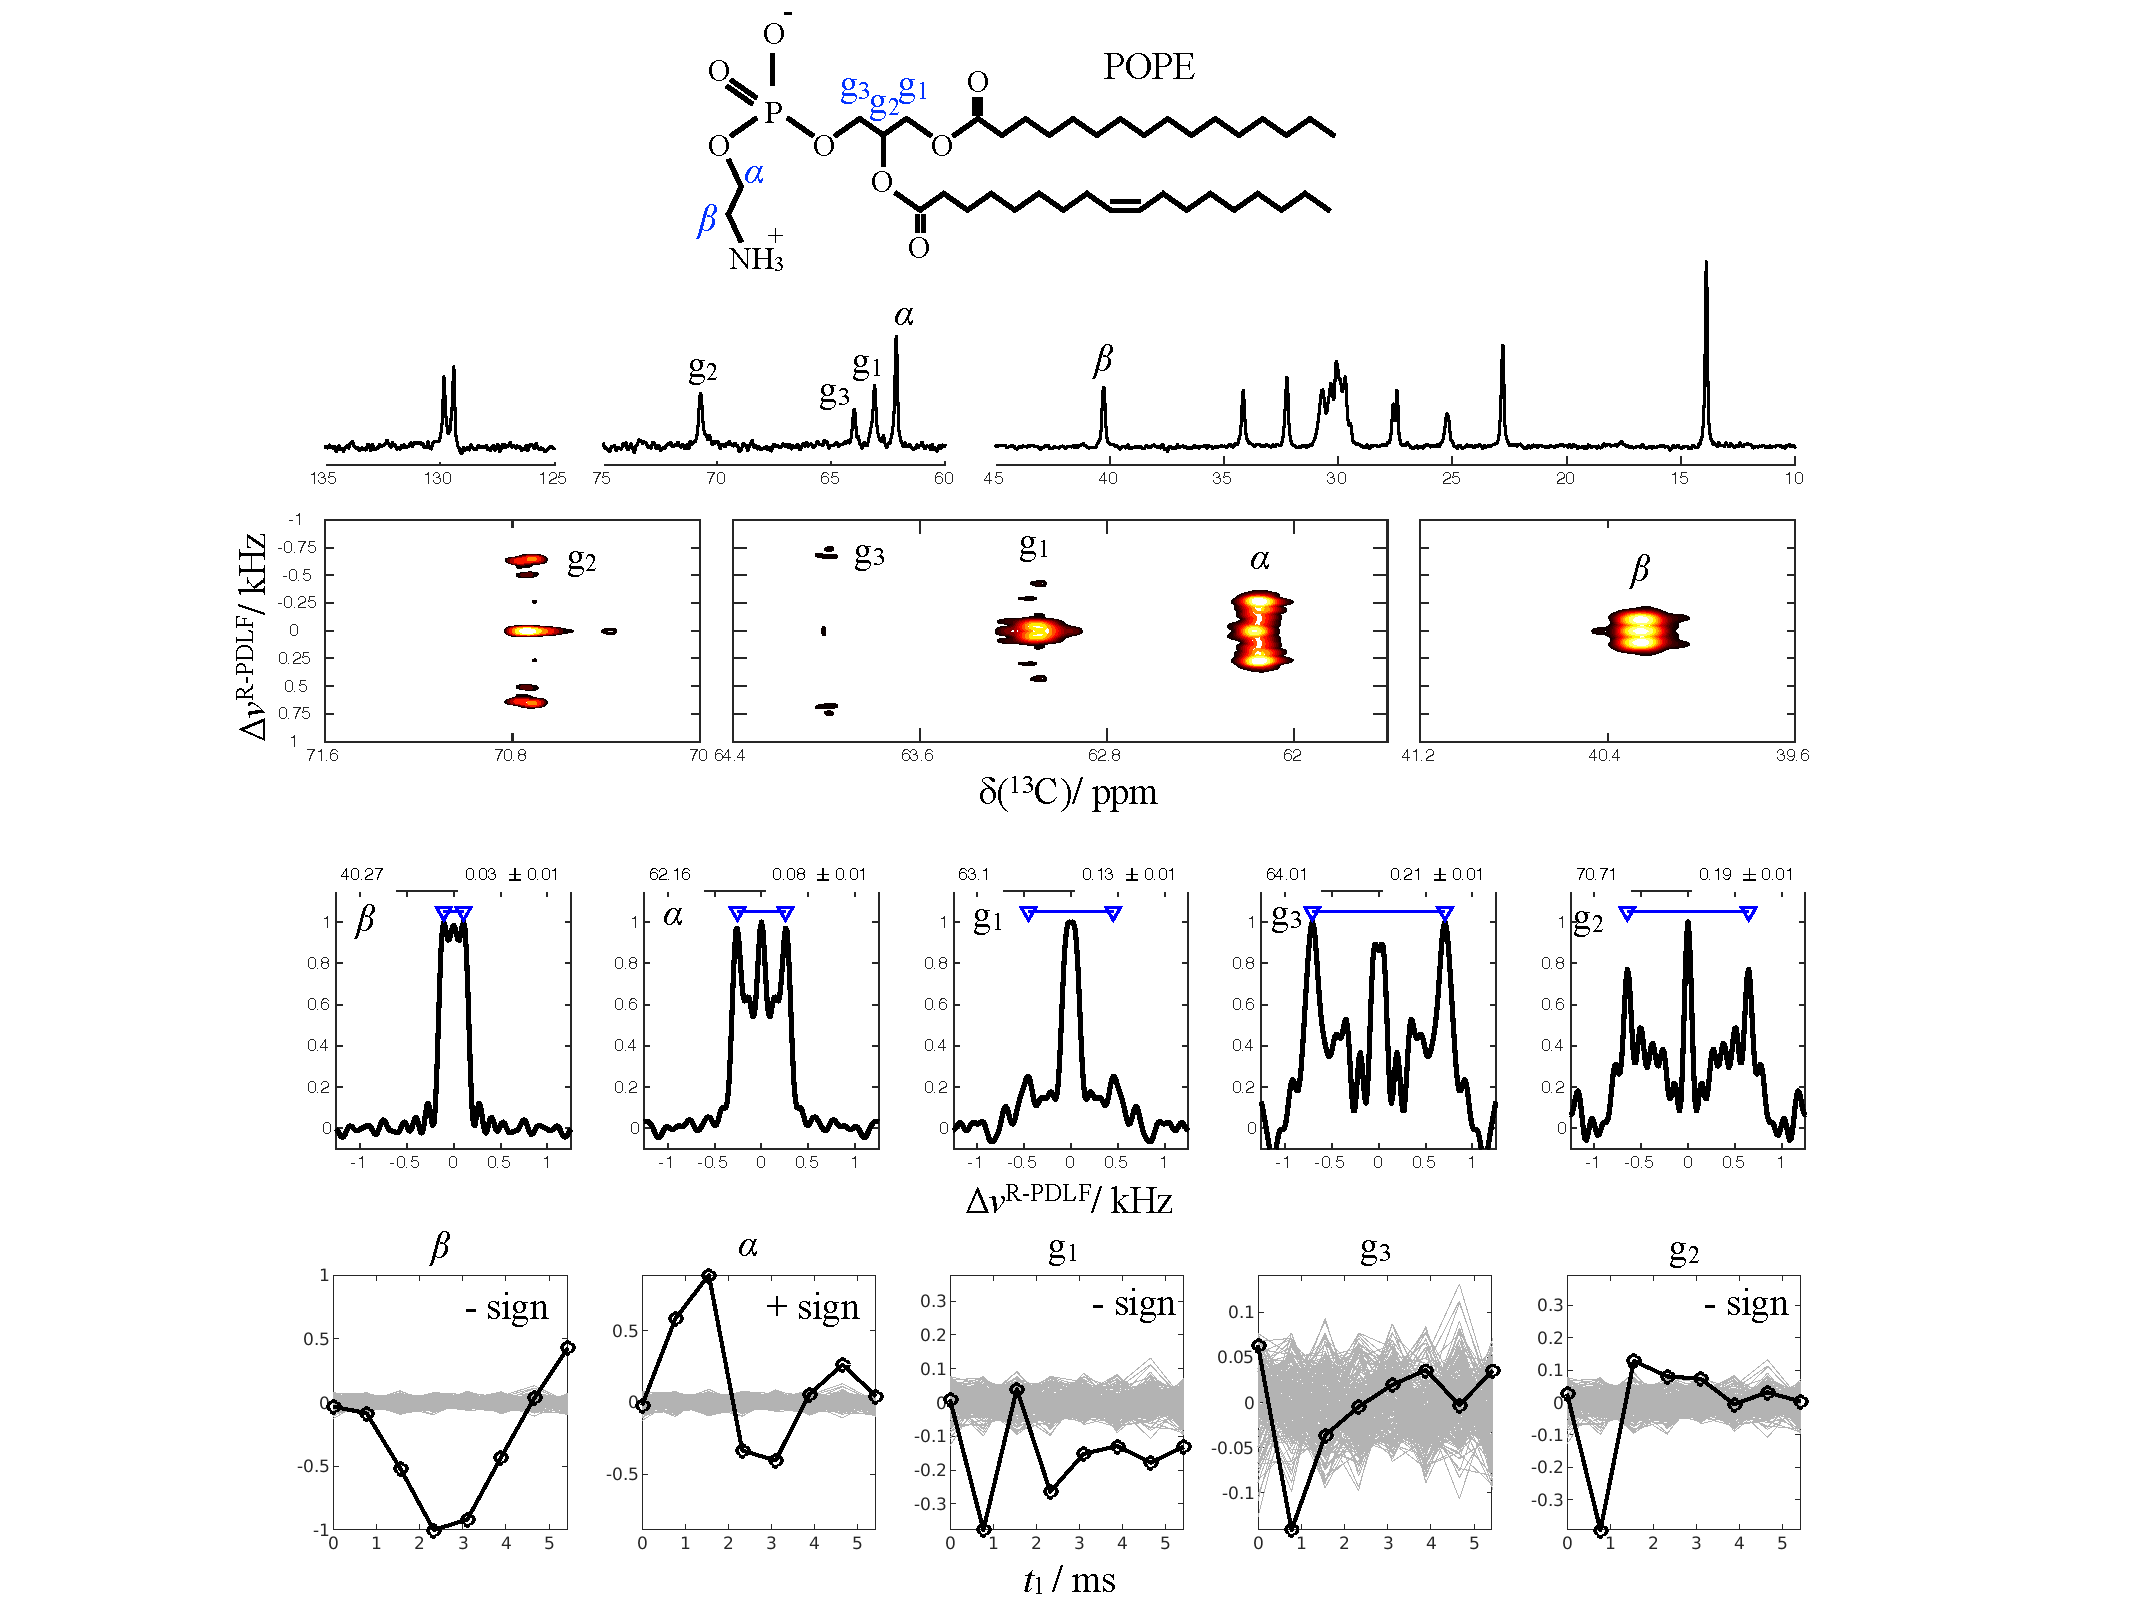
\includegraphics[width=0.8\textwidth]{./Figs/POPEexperiment.pdf}
  \caption{\label{POPEspectra}
    (A) Chemical structure of POPE with the labeling of headgroup and glycerol backbone carbons.
    (B) INEPT spectra from POPE sample with the headgroup and glycerol backbone peaks labeled.
    (C) 2D R-PDLF spectra
    (D) Dipolar sliced from the  2D R-PDLF spectra with the resulting order parameters on top of figures.
    (E) Experimetal S-DROSS curves giving signs of the order parameters.
  }
  \todo{A, B etc. labels to be put in the figure.}
\end{figure}

\begin{figure}[]
%  \centering
  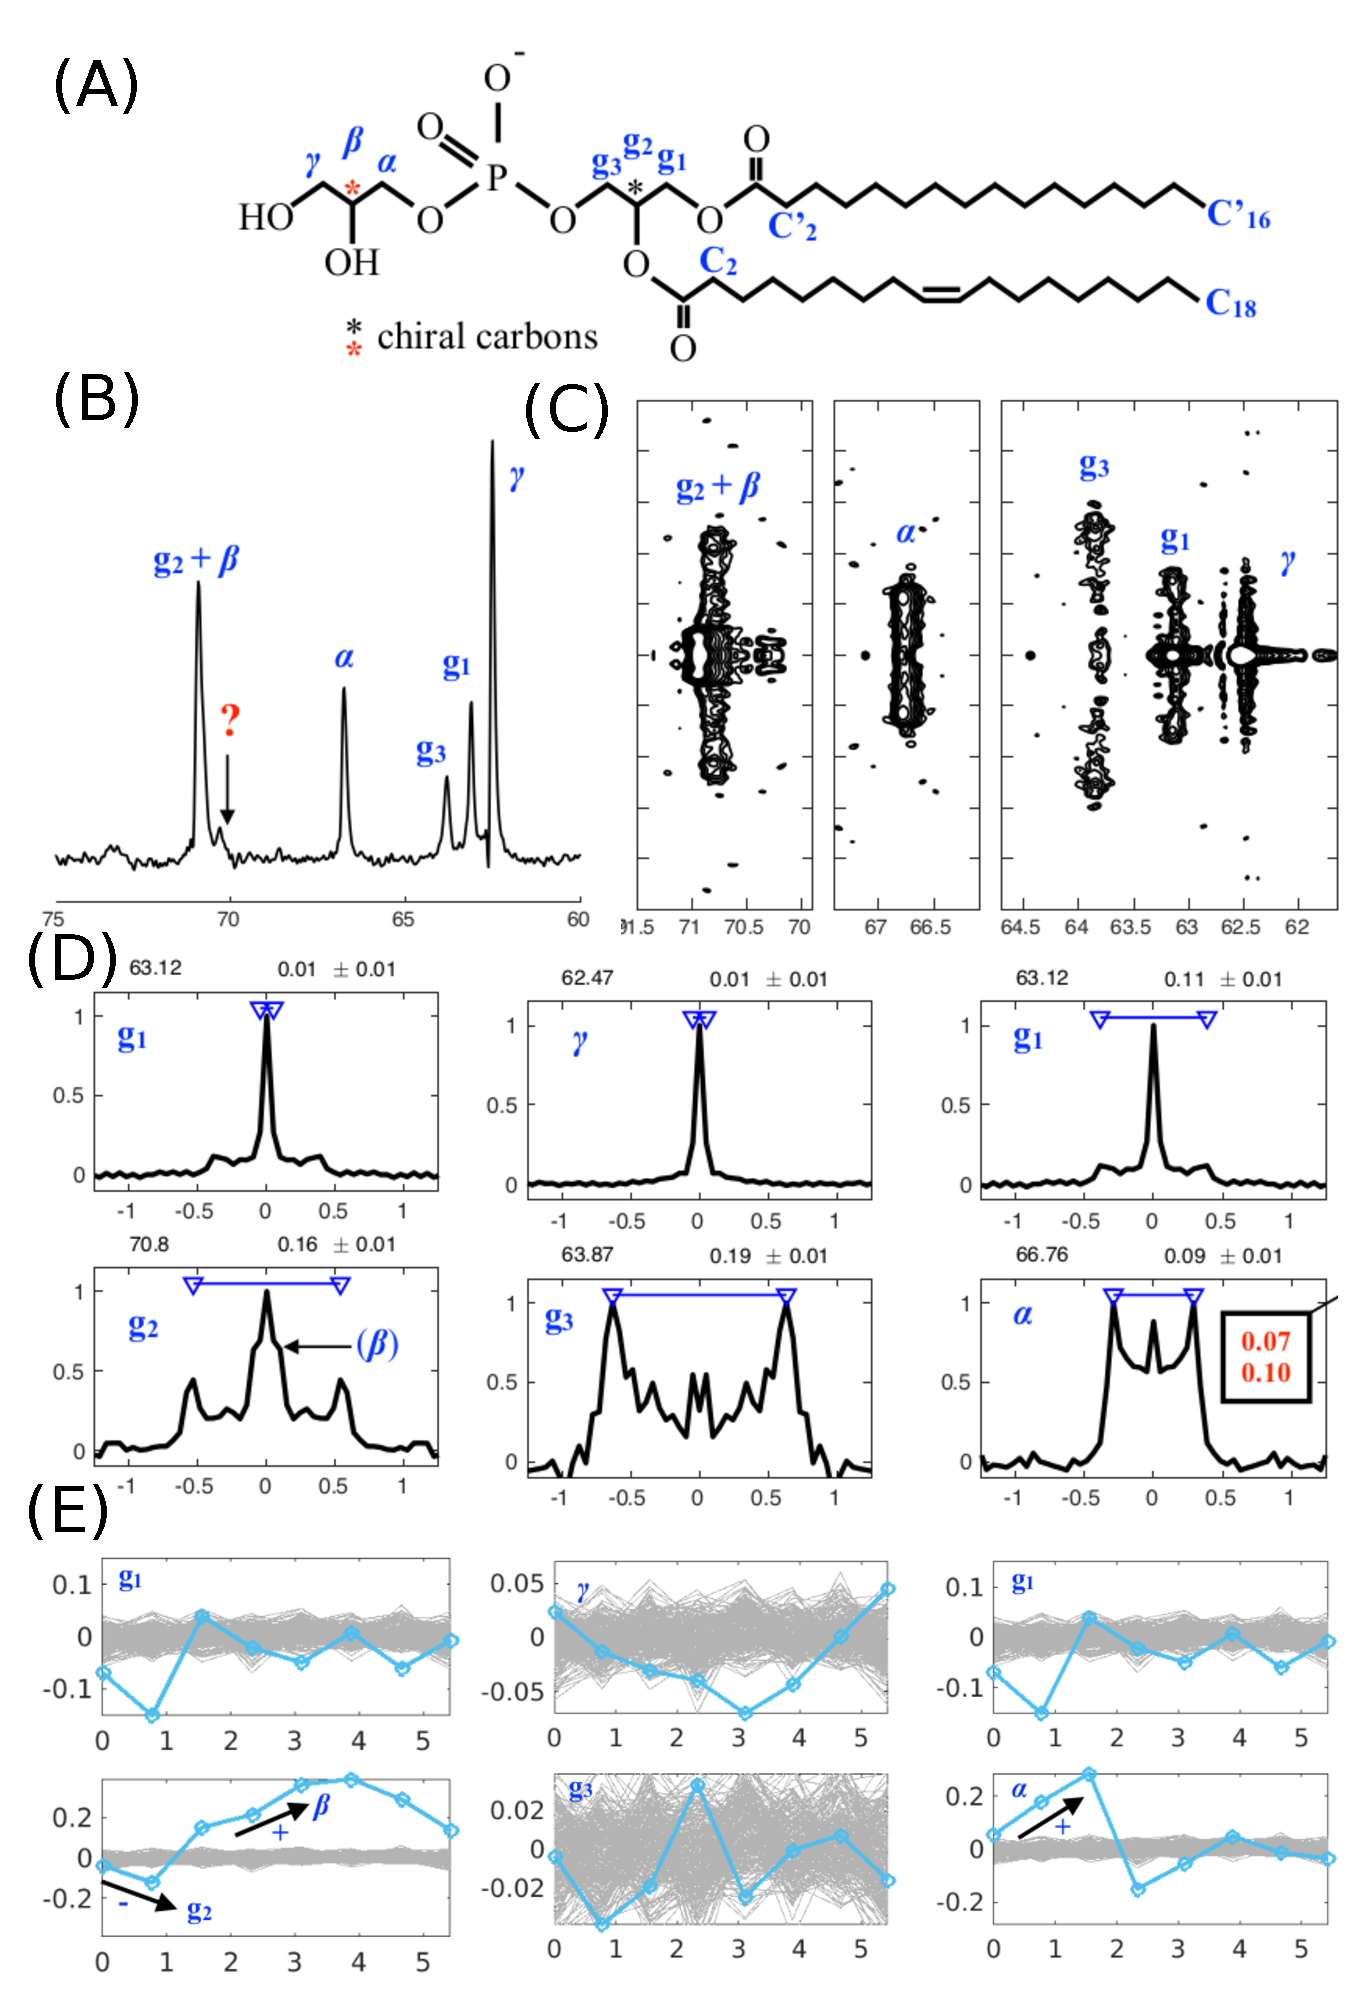
\includegraphics[width=0.8\textwidth]{./Figs/PGexpRPDLF.eps}
  \caption{\label{POPGspectra}
    (A) Chemical structure of POPG with the labeling of headgroup and glycerol backbone carbons.
    (B) INEPT spectra from POPG sample with the headgroup and glycerol backbone peaks labeled.
    (C) 2D R-PDLF spectra
    (D) Dipolar sliced from the  2D R-PDLF spectra with the resulting order parameters on top of figures.
    (E) Experimetal S-DROSS curves giving signs of the order parameters.
  }
\end{figure}

\begin{figure}[]
%  \centering
  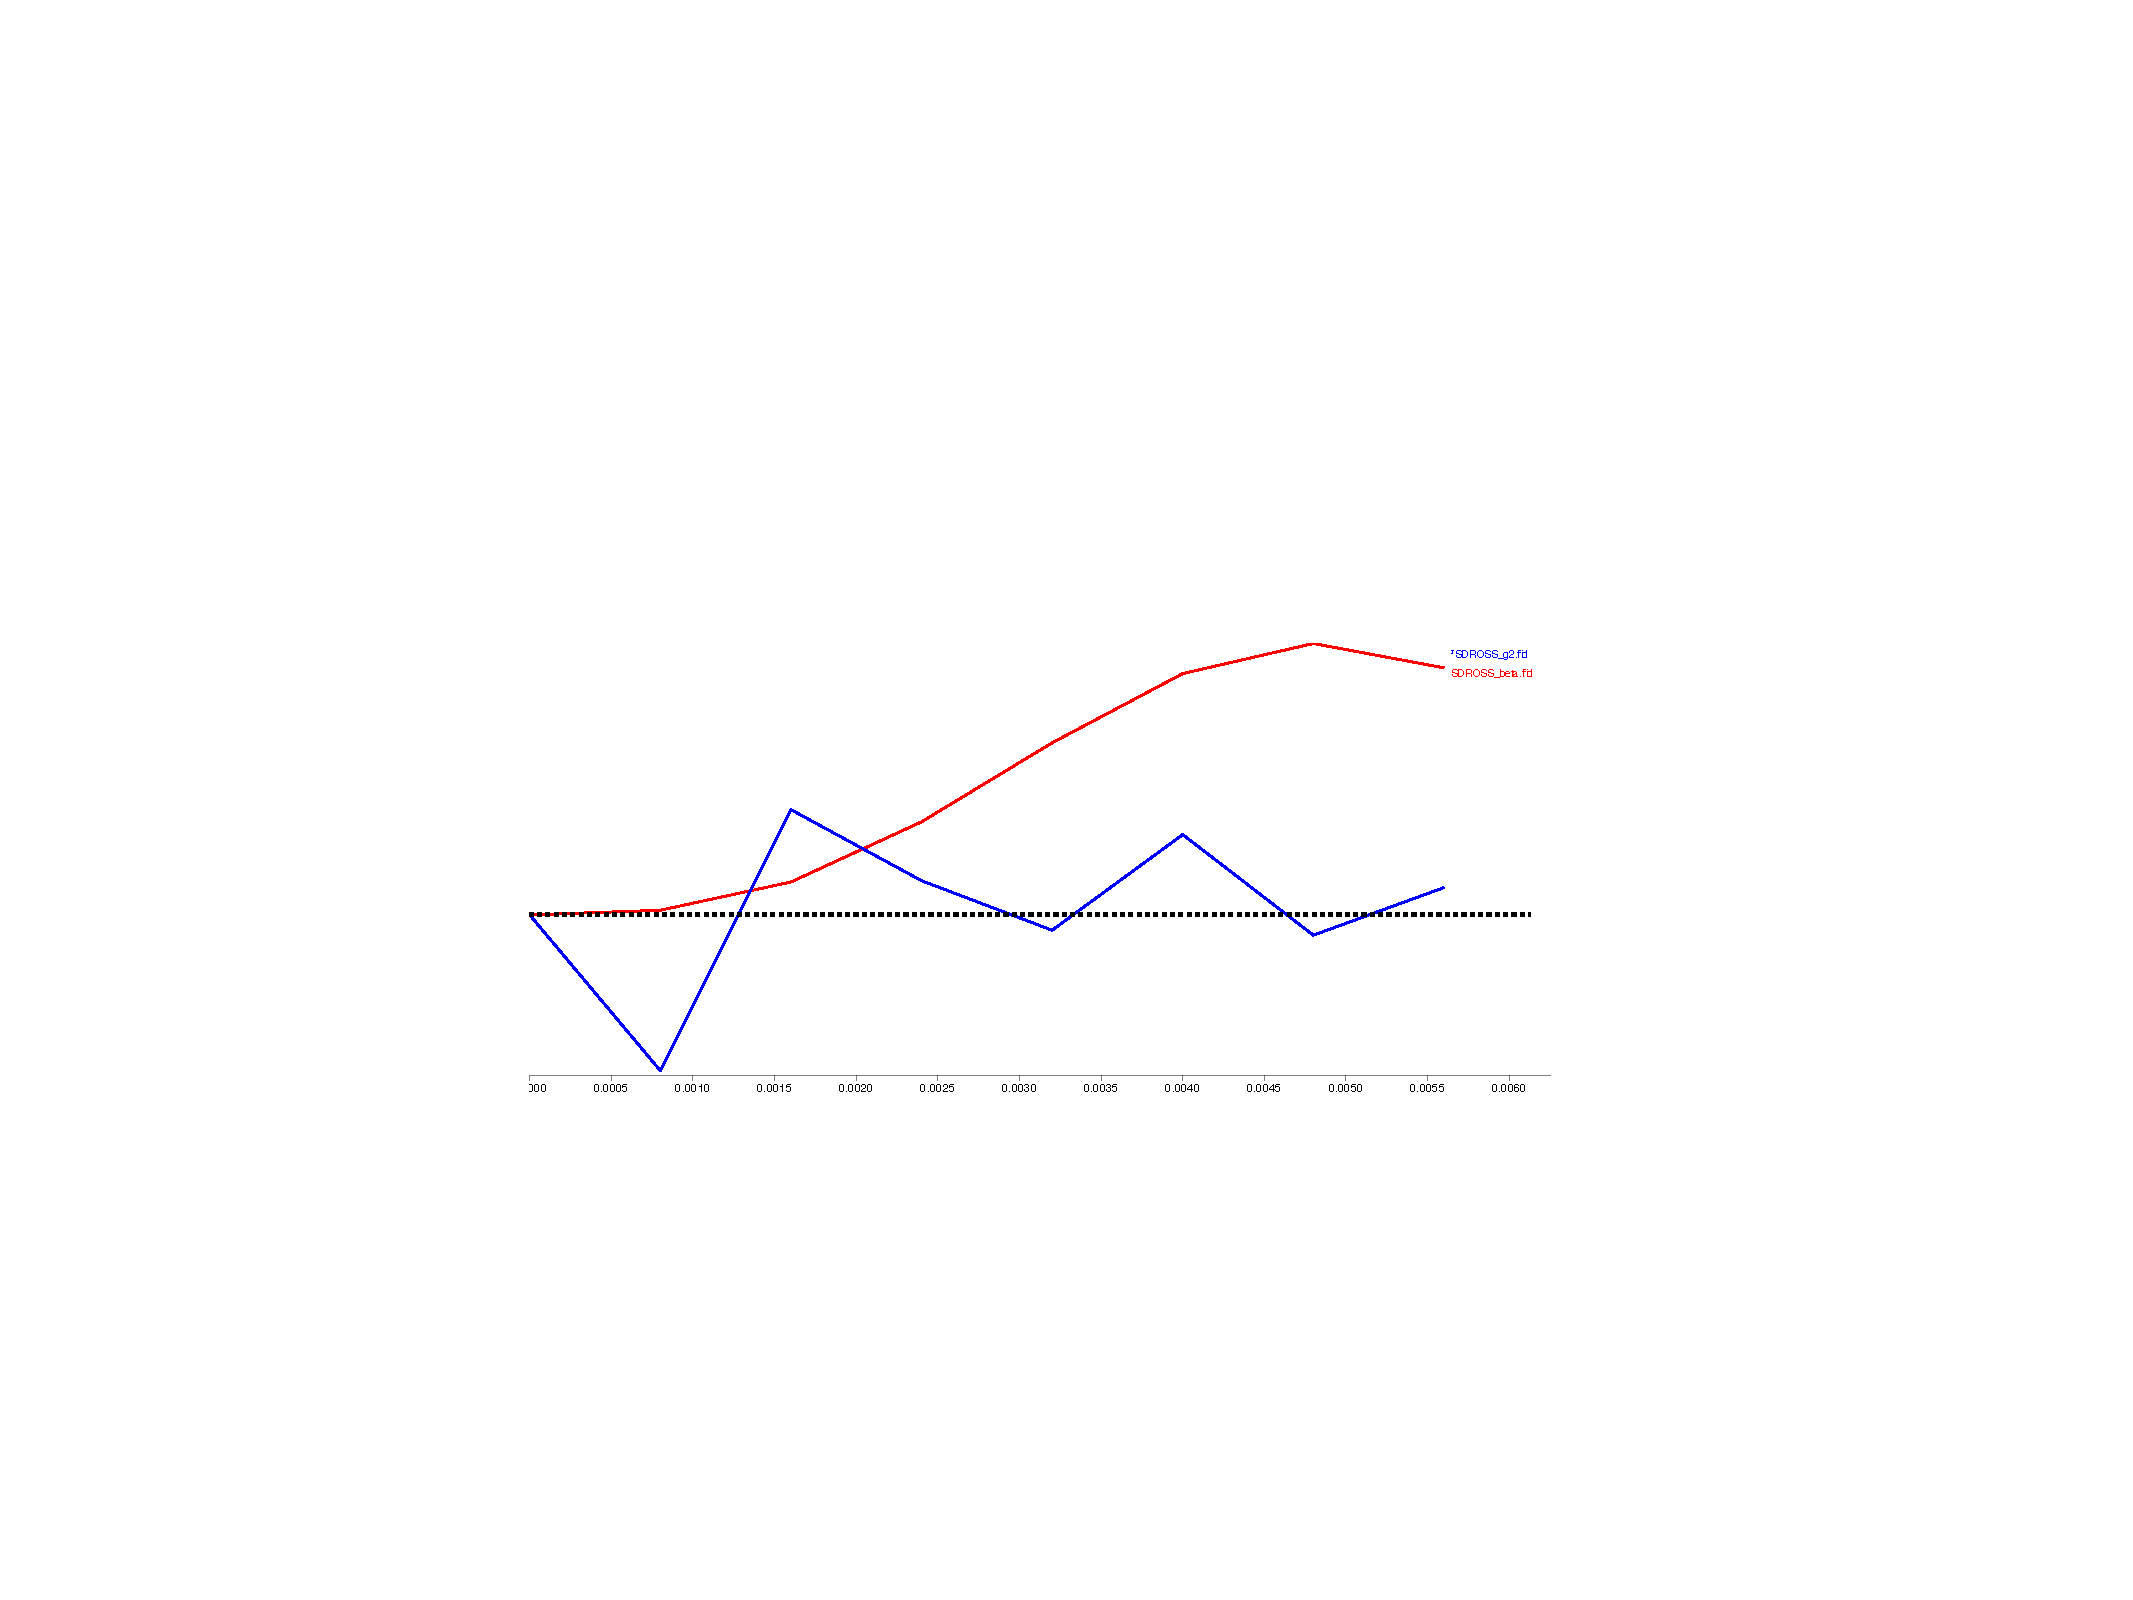
\includegraphics[width=0.8\textwidth]{./Figs/SIMPSON.pdf}
  \caption{\label{POPGsimpson}
    Simpson simulaton of S-DROSS curve of $\beta$-carbon of POPG.
  }
\end{figure}


\clearpage
\section{Evaluation of simulations against NMR experiments}
\subsection{Conformational ensembles of headgroup and glycerol backbone in PE and PG lipids}

The quality of PE and PG headgroup conformational ensembles in different simulations against NMR experiments is evaluated in figures \ref{HGorderParametersPE} and \ref{HGorderParametersPOPG} using C-H bond order parameters as in our previous studies for PC and PS lipids \cite{botan15,antila19}. Conclusions are the same for all lipids: None of the force fields correctly captures the lipid headgroup conformational ensembles, but CHARMM36 gives results closest to experiments.

It should be noted that the PG headgroup is biologically abundant R enantiomer in all simulations, while our $^{13}$C NMR experiments has a racemic mixture. Nevertheless, previous $^{2}$H NMR experiments comparing results between different enantiomers concluded that the structural differences between these are minor \cite{wohlgemuth80}.

%The poor performance of headgroup order parameters in Berger model can be probably explained by
%ring like structures seen in Fig. 6 in Ref. \citenum{mukhopadhyay04}, which is a typical feature
%for Berger based lipid force fields containing explicit hydrogen atoms in the head group \cite{zhao08,henin09,dahlberg10}.
%The poor performance of glycerol backbone of Slipids simulations is systemically observed also
%for other lipids in previous studies \cite{botan15,antila19}.
%\todo{Should we comment more the relative quality of different force fields and/or make the subjective force field ranking figures?
%https://github.com/NMRLipids/NMRlipidsIVPEandPG/issues/8}

\begin{figure}[]
  \centering
  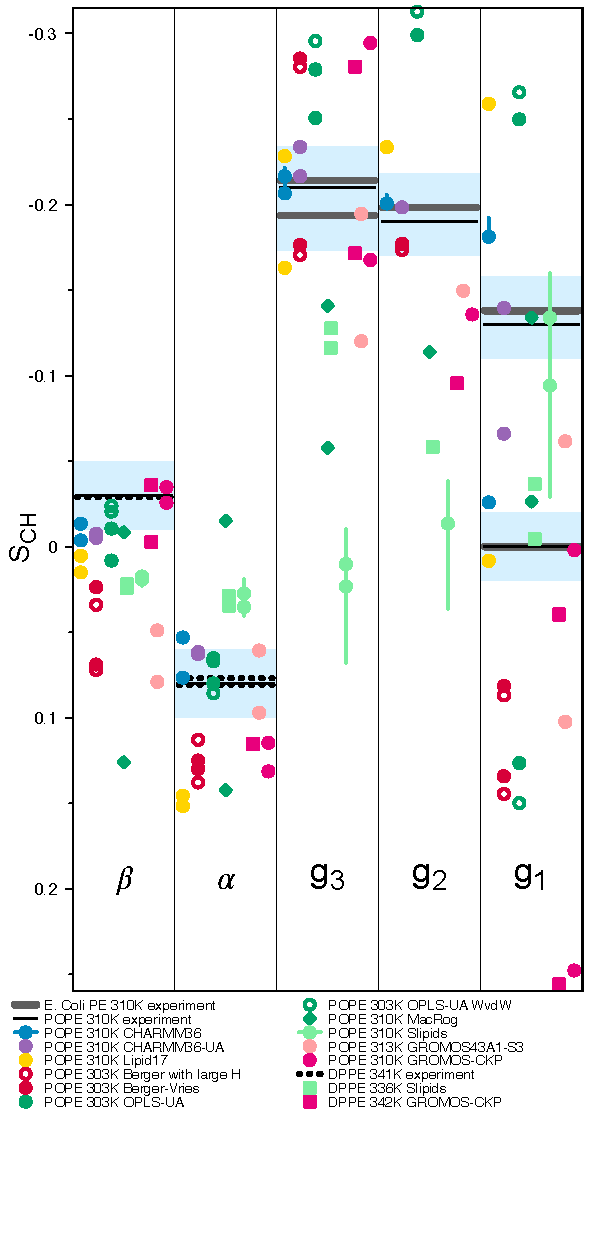
\includegraphics[width=9.0cm]{./Figs/HGorderparametersPE.pdf}
  \caption{\label{HGorderParametersPE}
    The headgroup and glycerol backbone order parameters of PE lipids
    from experiments (POPE and signs this work, DPPE from Ref.~\citenum{seelig76}
    and E.coliPE from Ref.~\citenum{gally81}) and simulations with different force fields.
  }
  \todo{This should be clarified as in NMRlipidsI and error bars should be added.
    Probably larger error bars for united atom models based on the report by Fuchs et al.
  } \\
  \todo{Lipid17 data should be updated to the one with correct dihedrals reported here https://github.com/NMRLipids/NMRlipidsIVPEandPG/issues/12\#issuecomment-756641407}
\end{figure}

\begin{figure}[!h]
  \centering
  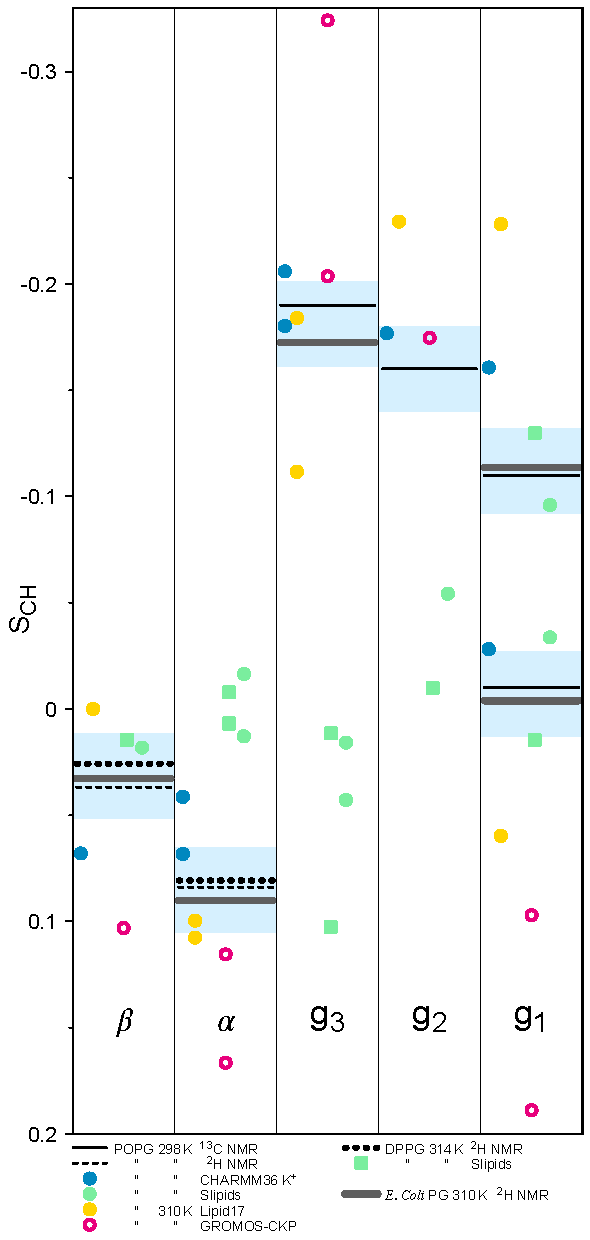
\includegraphics[width=9.0cm]{./Figs/HGorderparametersPG.pdf}
  \caption{\label{HGorderParametersPOPG}
    The headgroup and glycerol backbone order parameters of PG lipids
    from experiments (POPG and signs from this work and from Ref.~\citenum{borle85}, %contains 10mM of PIPES,
    DPPG with 100mM NaCl from Ref.~\citenum{wohlgemuth80},% contains 10mM PIPES and,
    and E.Coli PG results from Ref.~\citenum{gally81})
    and simulations with different force fields.
  }
   \todo{Lipid17 data should be updated to the one with correct dihedrals reported here https://github.com/NMRLipids/NMRlipidsIVPEandPG/issues/12\#issuecomment-756641407}
\end{figure}

\clearpage

\subsection{PC headgroup in mixtures with PE or PG lipids}
\begin{figure*}[]
  \centering
  \includegraphics[width=16.0cm]{./Figs/HGorderparametersPCvsPEPG.eps}
  \caption{\label{HGorderparametersPCvsPEPG}
    Modulation of POPC headgroup order parameters with increasing amount of POPE (left) and POPG (right) in bilayer
    from experiments at 298 K \cite{scherer87,macdonald87} and simulations with different force fields
    (temperatures listed in tables \ref{systemsMIX} and \ref{systemsMIX2} are between 298-310 K).
    Signs are determined as discussed in Refs. \citenum{botan15,ollila16}.
  }
\end{figure*}

Headgroup order parameters of PC lipids are unchanged upon addition
of zwitterionic lipids or cholesterol in experiments, but increase
upon addition of negatively charged PG or PS lipids because
headgroup dipole tilts more parallel to the membrane plane after incorporation
of negative charges into the membrane~\cite{seelig87, scherer87,antila18}.
The response of PC headgroup order parameters to the addition of PE or PG lipids
from different simulations is compared with experiments in figure~\ref{HGorderparametersPCvsPEPG}.
None of the simulations reproduce neither the experimentally observed increase in PC headgroup order parameters
with increasing amount of PG nor the related tilting of the headgroup more parallel with the membrane.
Similar observations in our previous work for PS lipids were explained by the overestimated counterion
binding affinity that neturalizes the effect of added negative charge \cite{antila19}.
All simulations except Berger-OPLS predict tilting of P-N headgroup outwards from the membrane and
decrease of PC headgroup order parameters upon addition of PE lipids.
These results are not in line with experiments where the PC headgroup order parameters are not affected by zwitterionic lipids \cite{scherer87}.
The good performance of Berger-OPLS simulations in here is surprising because
headgroup conformational enemble is not very close to experiments in this model and
the response of headgroup order parameters
to cholesterol was significantly overestimated by the Berger/H{\"o}ltje force field in our previous work \cite{botan15}.

In conclusion, more accurate force fields are needed to correctly simulate the interactions between different headgroups.

\clearpage
\subsection{PG headgroup in mixtures with PC lipids}
Changes in other than PC lipid headgroup with changing membrane composition are less
extensively characterized in the literature.
The $\beta$-carbon order parameter in PG headgroup increases
mildly \cite{macdonald87} or is unchanged~\cite{borle85} upon increasing amount
of PC lipids (Fig. \ref{HGorderparametersPGvsPCchange}), but experimental data from
$\alpha$-carbon is not available. Also the tested force fields predict very small changes
for the $\beta$-carbon order parameter, while the P-N vector tilt and its response to the
increased amount of PC varies significantly between force fields in figure \ref{HGorderparametersPGvsPCchange}. 
Therefore, more experimental data and more accurate force fields are still required
to resolve the PG conformational ensembles in mixtures with other lipids.
\begin{figure}[]
  \centering
  \includegraphics[width=8.0cm]{./Figs/HGorderparametersPGvsPCchange.eps}
  \caption{\label{HGorderparametersPGvsPCchange}
    Modulation of PG lipid headgroup order parameters with the increasing amount of PC in lipid bilayer
    from experiments at 298 K \cite{borle85,macdonald87} and simulations with different force fields at 310 K.
  }
\end{figure}

\clearpage
\subsection{Calcium binding to POPC:POPG mixtures}

The changes of headgroup order parameters in POPC:POPG mixtures upon addition of CaCl$_2$ between different simulations
and experiments \cite{borle85,macdonald87} are compared in figures \ref{changesWITHCaClPG} (molar ratio 1:1) and \ref{changesWITHCaClPG1PC4} (molar ratio 4:1).
The results are in line with our previous studies:
most force fields overestimate the calcium binding \cite{catte16,antila19}, but CHARMM36 with the NBfix correction underestimates the binding affinity \cite{antila19}, and the implicit inclusion of electronic polarizability using the electronic continuum correction (ECC) improves the results \cite{melcr18,melcr20}.


\begin{figure*}[]
  \centering
  \includegraphics[width=18.0cm]{./Figs/CHANGESwithCaClPG1PC1.eps}
  \caption{\label{changesWITHCaClPG}
    Modulation of headgroup order parameters of POPC ({\it left}) and POPG ({\it right}) in POPC:POPG (1:1)
    mixture upon addition of CaCl$_2$ in 298 K temperature from experiments \cite{borle85,macdonald87} and simulations.
    The $\beta$-carbon order parameter of POPC (dashed line on top left) is not directly measured but
    calculated from empirical relation $\Delta S_{\beta}=0.43\Delta S_{\alpha}$ \cite{akutsu81}.
    The changes with respect to the systems without CaCl$_2$ are shown for other data than
    for the $\alpha$-carbon of POPG for which experimental order parameter is not available.
    Calsium density distributions are shown in figure \ref{CAdensPG}.
    %(right) The headgroup order parameters of PG from PC:PG mixtures as a function CaCl$_2$
    %concentration from experiments \cite{borle85} and CHARMM36 simulations.
  }
\end{figure*}


\begin{figure}[]
  \centering
  \includegraphics[width=8.0cm]{./Figs/CAdensPG1PC1.eps}
  \caption{\label{CAdensPG}
    Calcium ion density profiles along membrane normal from simulations of POPC:POPG (1:1) mixtures with different force fields.
    The changes in the order parameters upon addition of CaCl$_2$ are compared with experiments in figure \ref{changesWITHCaClPG} in the main text.
  }
\end{figure}

\begin{figure*}[]
  \centering
  \includegraphics[width=18.0cm]{./Figs/CHANGESwithCaClPG1PC4.eps}
  \caption{\label{changesWITHCaClPG1PC4}
    Modulation of headgroup order parameters of POPC ({\it left}) and POPG ({\it right}) in POPC:POPG (4:1)
    mixture upon addition of CaCl$_2$ in 298 K temperature from experiments \cite{macdonald87} and simulations.
    The changes with respect to the systems without CaCl$_2$ are shown for other data than
    for the $\alpha$-carbon of POPG for which experimental order parameter is not available.
  }
  \todo{There is something wrong the Lipid17ecc data at 1M, a new simulation is coming.} \\
\end{figure*}

\begin{figure}[]
  \centering
  \includegraphics[width=8.0cm]{./Figs/CAdensPG1PC4.eps}
  \caption{\label{CAdensPG1PC4}
    Calcium ion density profiles along membrane normal from simulations of POPC:POPG (4:1) mixtures with different force fields.
  }
 \todo{Density profiles from Lipid17ecc data will be added when we have the new simulations at 1M.} \\
\end{figure}

\clearpage
\section{Changes in headgroup conformations upon addition of CaCl$_2$}


\begin{figure}[]
  \centering
  \includegraphics[width=12.0cm]{./Figs/DIHEDRALSlipid17eccWITHCaClPOPC.eps}
%  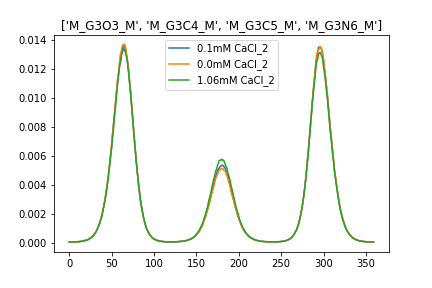
\includegraphics[width=6.0cm]{./Figs/dihedralFIGS/POPC_M_G3O3_M_M_G3C4_M_M_G3C5_M_M_G3N6_Mlipid17ecc.png}
%  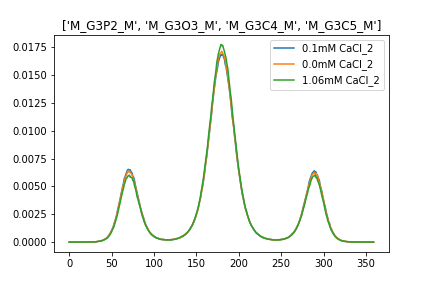
\includegraphics[width=6.0cm]{./Figs/dihedralFIGS/POPC_M_G3P2_M_M_G3O3_M_M_G3C4_M_M_G3C5_Mlipid17ecc.png}
%  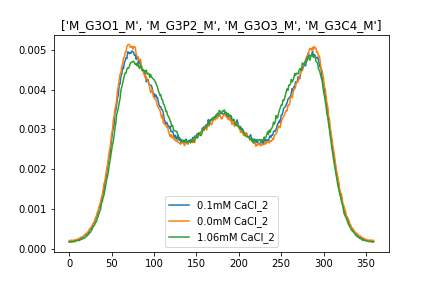
\includegraphics[width=6.0cm]{./Figs/dihedralFIGS/POPC_M_G3O1_M_M_G3P2_M_M_G3O3_M_M_G3C4_Mlipid17ecc.png}
%  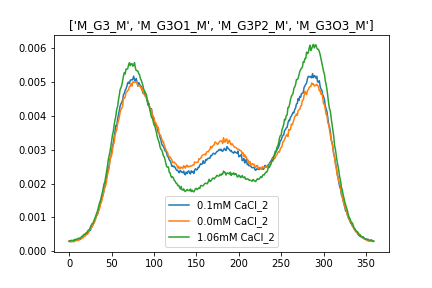
\includegraphics[width=6.0cm]{./Figs/dihedralFIGS/POPC_M_G3_M_M_G3O1_M_M_G3P2_M_M_G3O3_Mlipid17ecc.png}
%  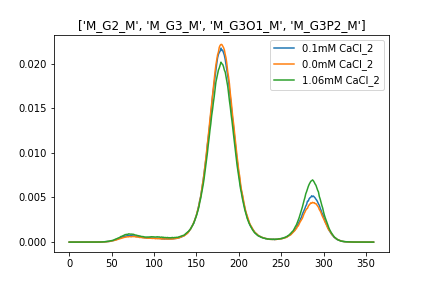
\includegraphics[width=6.0cm]{./Figs/dihedralFIGS/POPC_M_G2_M_M_G3_M_M_G3O1_M_M_G3P2_Mlipid17ecc.png}
%  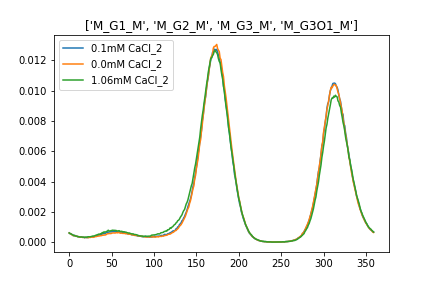
\includegraphics[width=6.0cm]{./Figs/dihedralFIGS/POPC_M_G1_M_M_G2_M_M_G3_M_M_G3O1_Mlipid17ecc.png}  
  \caption{\label{DIHSwithCAlipid17eccPOPC}
    Changes in POPC lipid17ecc dihedrals with increasing amount of CaCl$_2$.
  }
\end{figure}

\begin{figure}[]
  \centering
   \includegraphics[width=12.0cm]{./Figs/DIHEDRALScharmm36WITHCaClPOPC.eps}
%  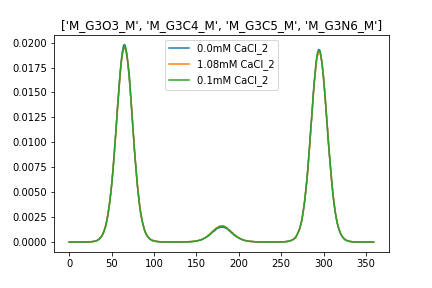
\includegraphics[width=6.0cm]{./Figs/dihedralFIGS/POPC_M_G3O3_M_M_G3C4_M_M_G3C5_M_M_G3N6_MCHARMM36.png}
%  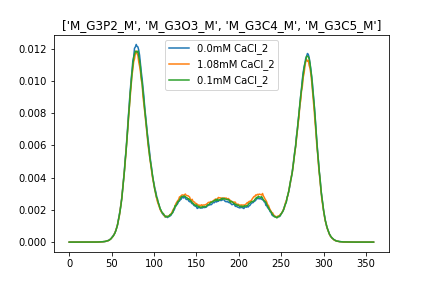
\includegraphics[width=6.0cm]{./Figs/dihedralFIGS/POPC_M_G3P2_M_M_G3O3_M_M_G3C4_M_M_G3C5_MCHARMM36.png}
%  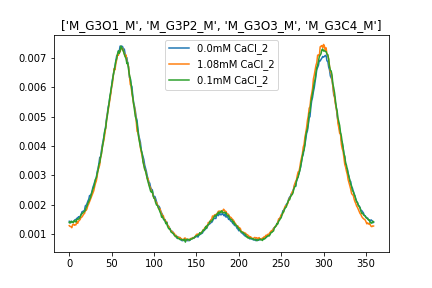
\includegraphics[width=6.0cm]{./Figs/dihedralFIGS/POPC_M_G3O1_M_M_G3P2_M_M_G3O3_M_M_G3C4_MCHARMM36.png}
%  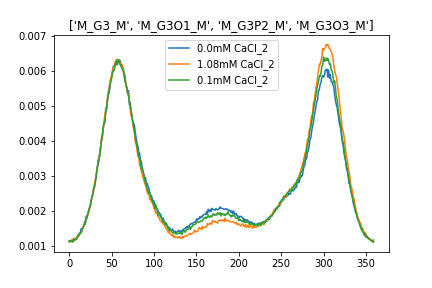
\includegraphics[width=6.0cm]{./Figs/dihedralFIGS/POPC_M_G3_M_M_G3O1_M_M_G3P2_M_M_G3O3_MCHARMM36.png}
%  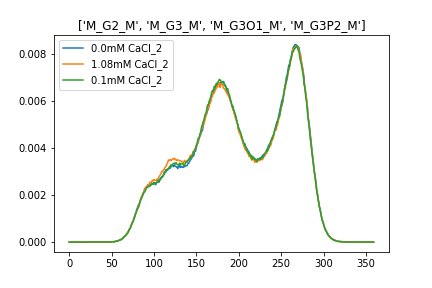
\includegraphics[width=6.0cm]{./Figs/dihedralFIGS/POPC_M_G2_M_M_G3_M_M_G3O1_M_M_G3P2_MCHARMM36.png}
%  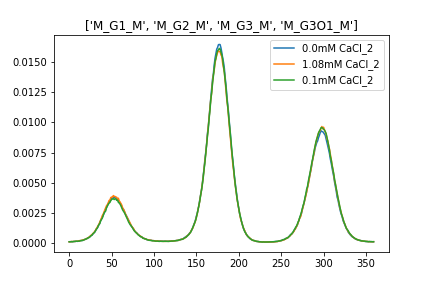
\includegraphics[width=6.0cm]{./Figs/dihedralFIGS/POPC_M_G1_M_M_G2_M_M_G3_M_M_G3O1_MCHARMM36.png}  
  \caption{\label{DIHSwithCAcharmm36POPC}
    Changes in POPC CHARMM36 dihedrals with increasing amount of CaCl$_2$.
  }
\end{figure}


%\begin{figure}[]
%  \centering
%  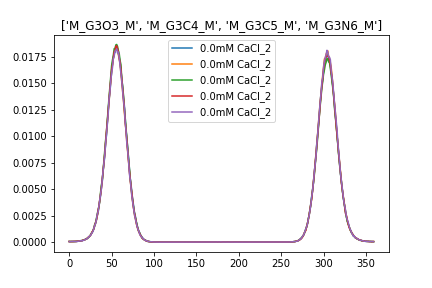
\includegraphics[width=6.0cm]{./Figs/dihedralFIGS/POPC_M_G3O3_M_M_G3C4_M_M_G3C5_M_M_G3N6_MSlipids.png}
%  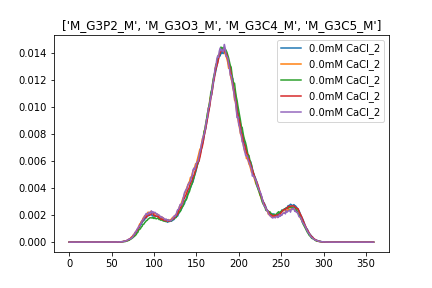
\includegraphics[width=6.0cm]{./Figs/dihedralFIGS/POPC_M_G3P2_M_M_G3O3_M_M_G3C4_M_M_G3C5_MSlipids.png}
%  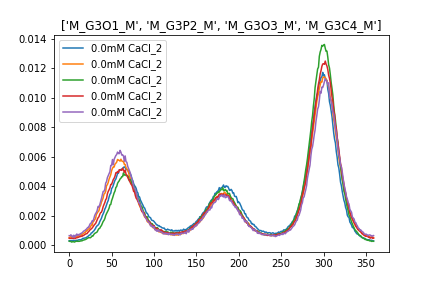
\includegraphics[width=6.0cm]{./Figs/dihedralFIGS/POPC_M_G3O1_M_M_G3P2_M_M_G3O3_M_M_G3C4_MSlipids.png}
%  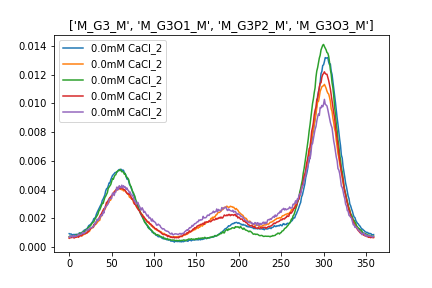
\includegraphics[width=6.0cm]{./Figs/dihedralFIGS/POPC_M_G3_M_M_G3O1_M_M_G3P2_M_M_G3O3_MSlipids.png}
%  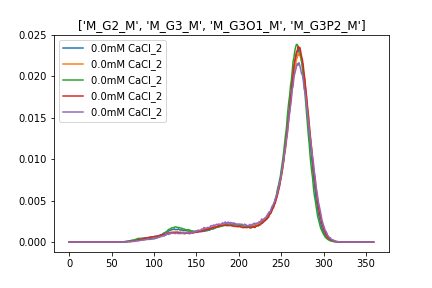
\includegraphics[width=6.0cm]{./Figs/dihedralFIGS/POPC_M_G2_M_M_G3_M_M_G3O1_M_M_G3P2_MSlipids.png}
%  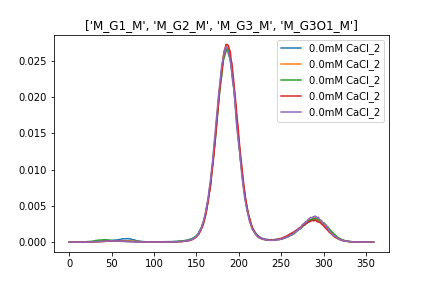
\includegraphics[width=6.0cm]{./Figs/dihedralFIGS/POPC_M_G1_M_M_G2_M_M_G3_M_M_G3O1_MSlipids.png}  
%  \caption{\label{DIHSwithCA}
%    Changes in POPC Slipids dihedrals with increasing amount of CaCl$_2$.
%  }
%\end{figure}

\begin{figure}[]
  \centering
  \includegraphics[width=16.0cm]{./Figs/DIHEDRALSslipidsWITHCaClPOPG.eps}
  %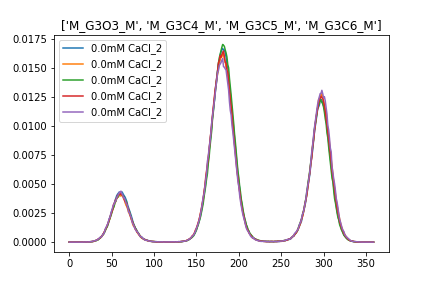
\includegraphics[width=6.0cm]{./Figs/dihedralFIGS/POPG_M_G3O3_M_M_G3C4_M_M_G3C5_M_M_G3C6_MSlipids.png}
  %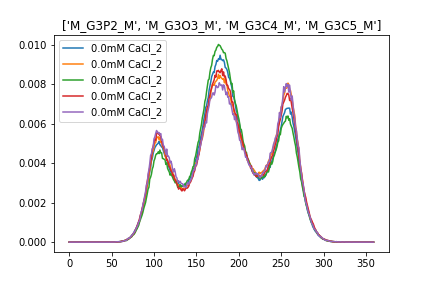
\includegraphics[width=6.0cm]{./Figs/dihedralFIGS/POPG_M_G3P2_M_M_G3O3_M_M_G3C4_M_M_G3C5_MSlipids.png}
  %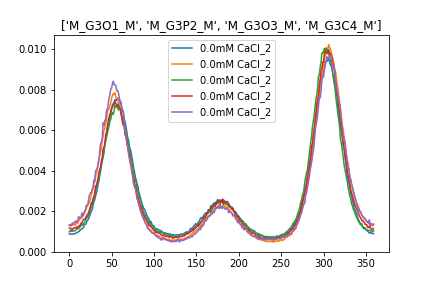
\includegraphics[width=6.0cm]{./Figs/dihedralFIGS/POPG_M_G3O1_M_M_G3P2_M_M_G3O3_M_M_G3C4_MSlipids.png}
  %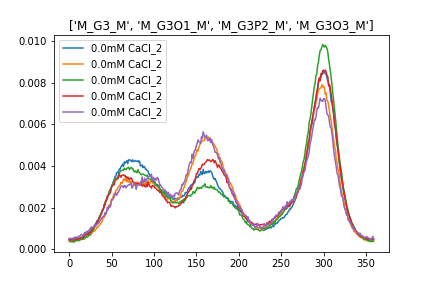
\includegraphics[width=6.0cm]{./Figs/dihedralFIGS/POPG_M_G3_M_M_G3O1_M_M_G3P2_M_M_G3O3_MSlipids.png}
  %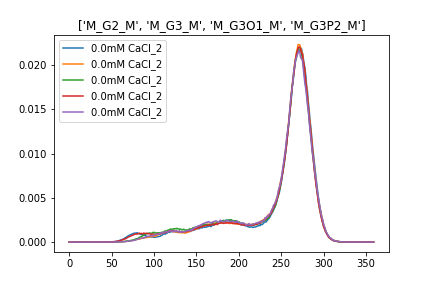
\includegraphics[width=6.0cm]{./Figs/dihedralFIGS/POPG_M_G2_M_M_G3_M_M_G3O1_M_M_G3P2_MSlipids.png}
  %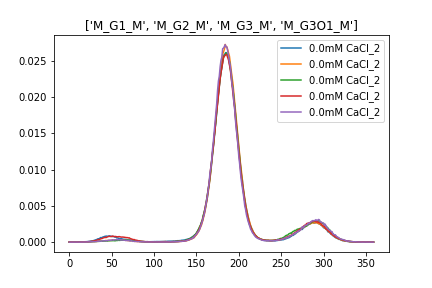
\includegraphics[width=6.0cm]{./Figs/dihedralFIGS/POPG_M_G1_M_M_G2_M_M_G3_M_M_G3O1_MSlipids.png}  
  \caption{\label{DIHSwithCAslipidsPOPG}
    Changes in POPG Slipids dihedrals with increasing amount of CaCl$_2$.
  }
\end{figure}

%\begin{figure}[]
%  \centering
%  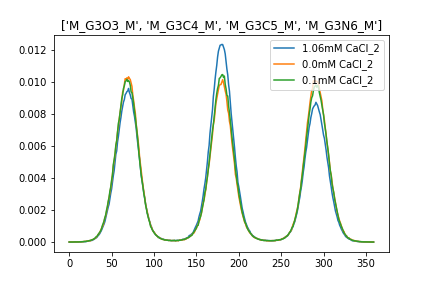
\includegraphics[width=6.0cm]{./Figs/dihedralFIGS/POPC_M_G3O3_M_M_G3C4_M_M_G3C5_M_M_G3N6_Mlipid17.png}
%  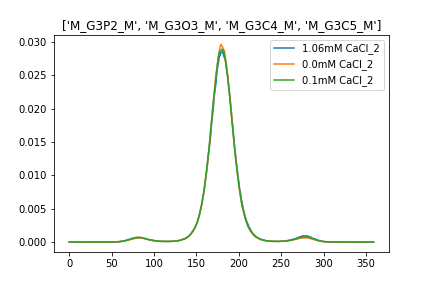
\includegraphics[width=6.0cm]{./Figs/dihedralFIGS/POPC_M_G3P2_M_M_G3O3_M_M_G3C4_M_M_G3C5_Mlipid17.png}
%  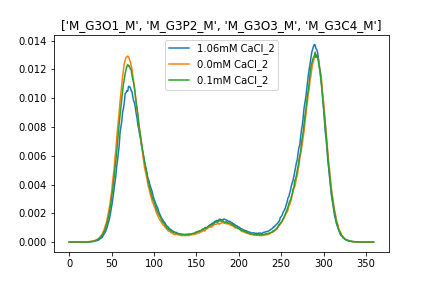
\includegraphics[width=6.0cm]{./Figs/dihedralFIGS/POPC_M_G3O1_M_M_G3P2_M_M_G3O3_M_M_G3C4_Mlipid17.png}
%  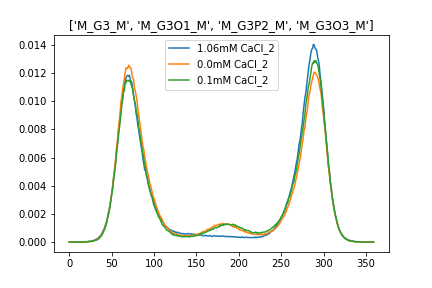
\includegraphics[width=6.0cm]{./Figs/dihedralFIGS/POPC_M_G3_M_M_G3O1_M_M_G3P2_M_M_G3O3_Mlipid17.png}
%  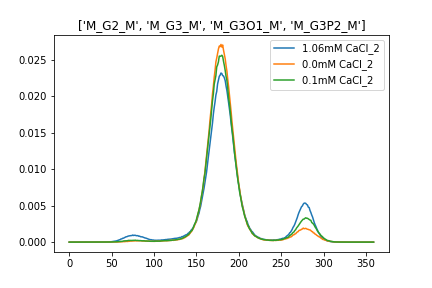
\includegraphics[width=6.0cm]{./Figs/dihedralFIGS/POPC_M_G2_M_M_G3_M_M_G3O1_M_M_G3P2_Mlipid17.png}
%  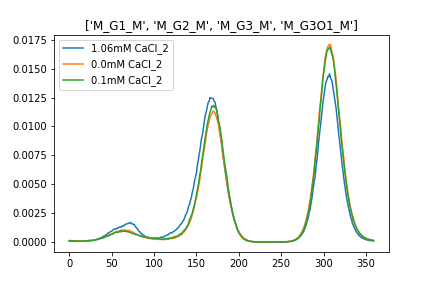
\includegraphics[width=6.0cm]{./Figs/dihedralFIGS/POPC_M_G1_M_M_G2_M_M_G3_M_M_G3O1_Mlipid17.png}  
%  \caption{\label{DIHSwithCA}
%    Changes in POPC lipid17 dihedrals with increasing amount of CaCl$_2$.
%  }
%\end{figure}

\begin{figure}[]
  \centering
  \includegraphics[width=16.0cm]{./Figs/DIHEDRALSlipid17WITHCaClPOPG.eps}
  %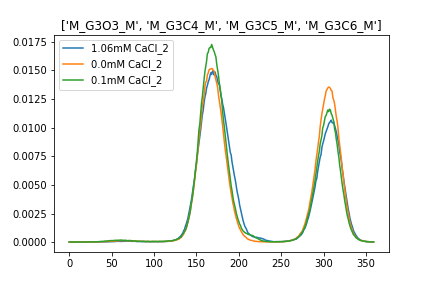
\includegraphics[width=6.0cm]{./Figs/dihedralFIGS/POPG_M_G3O3_M_M_G3C4_M_M_G3C5_M_M_G3C6_Mlipid17.png}
  %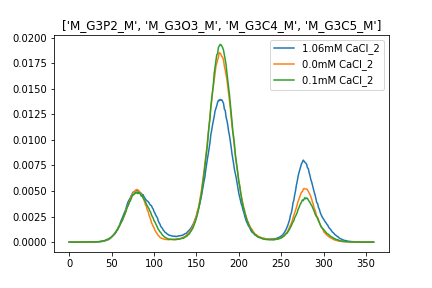
\includegraphics[width=6.0cm]{./Figs/dihedralFIGS/POPG_M_G3P2_M_M_G3O3_M_M_G3C4_M_M_G3C5_Mlipid17.png}
  %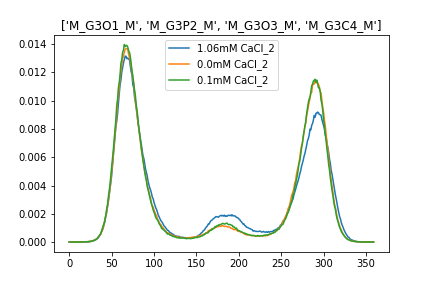
\includegraphics[width=6.0cm]{./Figs/dihedralFIGS/POPG_M_G3O1_M_M_G3P2_M_M_G3O3_M_M_G3C4_Mlipid17.png}
  %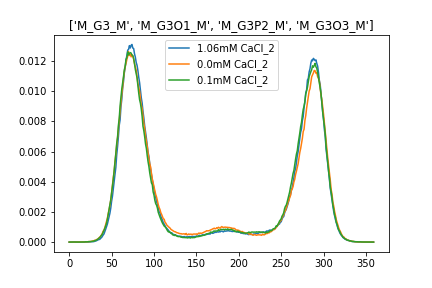
\includegraphics[width=6.0cm]{./Figs/dihedralFIGS/POPG_M_G3_M_M_G3O1_M_M_G3P2_M_M_G3O3_Mlipid17.png}
  %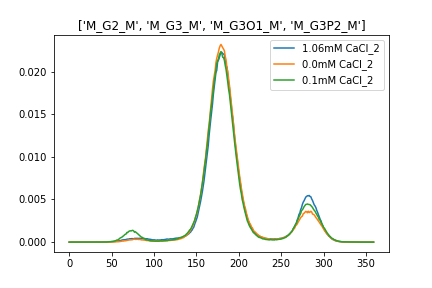
\includegraphics[width=6.0cm]{./Figs/dihedralFIGS/POPG_M_G2_M_M_G3_M_M_G3O1_M_M_G3P2_Mlipid17.png}
  %\includegraphics[width=6.0cm]{./Figs/dihedralFIGS/POPG_M_G1_M_M_G2_M_M_G3_M_M_G3O1_Mlipid17.png}  
  \caption{\label{DIHSwithCAlipid17POPG}
    Changes in POPG lipid17 dihedrals with increasing amount of CaCl$_2$.
  }
\end{figure}


%\begin{figure}[]
%  \centering
%  \includegraphics[width=6.0cm]{./Figs/dihedralFIGS/POPG_M_G3O3_M_M_G3C4_M_M_G3C5_M_M_G3C6_Mlipid17ecc.png}
%  \includegraphics[width=6.0cm]{./Figs/dihedralFIGS/POPG_M_G3P2_M_M_G3O3_M_M_G3C4_M_M_G3C5_Mlipid17ecc.png}
%  \includegraphics[width=6.0cm]{./Figs/dihedralFIGS/POPG_M_G3O1_M_M_G3P2_M_M_G3O3_M_M_G3C4_Mlipid17ecc.png}
%  \includegraphics[width=6.0cm]{./Figs/dihedralFIGS/POPG_M_G3_M_M_G3O1_M_M_G3P2_M_M_G3O3_Mlipid17ecc.png}
%  \includegraphics[width=6.0cm]{./Figs/dihedralFIGS/POPG_M_G2_M_M_G3_M_M_G3O1_M_M_G3P2_Mlipid17ecc.png}
%  \includegraphics[width=6.0cm]{./Figs/dihedralFIGS/POPG_M_G1_M_M_G2_M_M_G3_M_M_G3O1_Mlipid17ecc.png}  
%  \caption{\label{DIHSwithCA}
%    Changes in POPG lipid17ecc dihedrals with increasing amount of CaCl$_2$.
%  }
%\end{figure}




\clearpage
\section{Simulated systems}

The simulated systems of pure PE and PG bilayers without additional ions
are listed in Tables~\ref{systemsPE} and \ref{systemsPG},
and lipid mixtures with additional ions in Tables~\ref{systemsMIX} and \ref{systemsMIX2}.
the simulation data are indexed in a
searchable database available at \url{www.nmrlipids.fi},
and in the NMRlipids/MATCH repository (\url{github.com/NMRlipids/MATCH}).
The large set of MD simulation data was analysed using the development version of NMRlipids databank.
Unique naming convention for lipid atoms in each force field was defined using the mapping files
and analysis for all simulations indexed in NMRlipids databank manner were performed
using Python codes.

The C--H bond order parameters were calculated directly
from the carbon and hydrogen positions using the definition
\begin{equation}
S_{\rm CH}=\frac{1}{2}\left\langle 3\cos^2\theta -1 \right\rangle,
\end{equation}
where $\theta$ is the angle between the C--H bond and the membrane normal
(taken to align with $z$, with bilayer periodicity in the $xy$-plane).
Angular brackets denote average over all sampled configurations.
The order parameters were first calculated averaging over time separately
for each lipid in the system. The average and
the standard error of the mean were then calculated over different lipids.
Python programs that use the MDAnalysis library \cite{agrawal11,gowers16}
used for all atom simulations are available in Ref.~\citenum{MATCHgit}
(\texttt{scripts/calcOrderParameters.py}). For united atom simulations, the trajectories with hydrogens having ideal geometry were constructed first using either \texttt{buildH} program~\cite{buildH} or (\texttt{scratch/opAAUA\_prod.py}) in  Ref.~\citenum{MATCHgit}, and the order parameters were then calculated from these trajectories. This approach has been tested against trajectories with explicit hydrogens and the deviations in order parameters are small \cite{buildH,piggot17}.\\
%\todo{BuildH program is now cited with a direct link to the GitHub repo. I think that a release to Zenodo would be nice in the final publication.}\\
The number density profiles of ions were calculated using the \texttt{gmx density} tool of the GROMACS sofware package \cite{gromacsMANUAL}.


%\begin{table*}[htb]
%
\begin{sidewaystable*}[!p]
  \centering
  \caption{List of MD simulations with PE lipids.
    % The salt concentrations calculated as [salt]=N$_{\rm c} \times$[water]\,/\,N$_{\rm w}$, where [water]\,=\,55.5~M.
    % these correspond the concentrations reported in the experiments by Akutsu et al.~\cite{akutsu81}.
    % The lipid force fields named as in our previous work~\cite{botan15}.
  }\label{systemsPE}
  \begin{minipage}[t]{\textwidth}
    \begin{tabular}{l c c r r r r r r c c}
      %\hline
      % some footnotes are not visible in typeset-MS (pdf)
      lipid/counter-ions & force field for lipids / ions  & NaCl (M) & \footnote{Number of lipid molecules with largest mole fraction}N$_{\rm l}$   &  \footnote{Number of water molecules}N$_{\rm w}$   & \footnote{Number of additional cations}N$_{\rm c}$   & \footnote{Simulation temperature}T (K)  & \footnote{Total simulation time}t$_{{\rm sim}}$(ns) & \footnote{Time used for analysis}t$_{{\rm anal}}$ (ns) &   \footnote{Reference for simulation files}files\\
      \hline
      POPE  & CHARMM36 \cite{??}           &0       & 144	& 5760  &0    & 310  & 500          & 400          & \cite{charmm36POPEfiles} \\
      POPE  & CHARMM36 \cite{??}           & 0      & 500       & 25000 & 0   &  310  & 500 & 100 & \cite{POPEcharmm} \\
      POPE  & CHARMM36 \cite{??}           & 0.11   & 500       & 25000 & 50  &  310  & 500 & 100 & \cite{POPEcharmm150mMNaCl} \\
      POPE  & CHARMM36ua \cite{??}         &0       & 336	& 15254 &0    & 310  & 2$\times$200 & 2$\times$100 & \cite{charmm36uaPOPEfiles}  \\
      \hline
      DPPE  & Slipids \cite{jambeck12b}    &0    & 288 	& 9386  &0    & 336  & 200 & 100 & \cite{slipidsDPPEfiles}  \\
      POPE  & Slipids \cite{jambeck12b} &0    & 336	& ?     &0    & 310  & 2$\times$200 &  2$\times$100 & \cite{slipidsPOPEfiles}  \\
      POPE  & Slipids \cite{jambeck12b}            & 0    & 500 & 25000 & 0   &  310  & 500 & 100 & \cite{POPEslipids} \\
      POPE  & Slipids / {\AA}qvist \cite{jambeck12b,aqvist90}  & 0.11 & 500 & 25000 & 50  &  310  & 500 & 100 & \cite{POPEslipids150mMNaCl} \\
      \hline
      DPPE  & GROMOS-CKP    \cite{??}      &0    & 128	& 3655  &0    & 342  & 2$\times$500 & 2$\times$400 & \cite{gromosCKPdppe} \\
      POPE  & GROMOS-CKP    \cite{??}      &0    & 128	& 3552  &0    & 313  & 2$\times$500 & 2$\times$400 & \cite{gromosCKPpope} \\
      POPE  & GROMOS-CKP    \cite{??}      &0    & 500	& 25000 &0    & 310  & 500 & 100 & \cite{gromosCKPpopeT310} \\
      POPE  & GROMOS-CKP    \cite{??}      &0.11 & 500	& 25000 &50   & 310  & 500 & 100 & \cite{gromosCKPpopeT310150mMNaCl} \\
      DOPE  & GROMOS-CKP    \cite{??}      &0    & 128	& 4789  &0    & 271  & 2$\times$500 & 2$\times$400 & \cite{gromosCKPdope} \\
      \hline
      POPE  & GROMOS 43A1-S3 \cite{??}     &0    & 128	& 3552     &0    & 313  & 2$\times$200 & 2$\times$100 & \cite{gromos43a1s3POPEfiles}  \\
      \hline
      POPE  & OPLS-UA vdW on H \cite{??}   &0    & 128	& 3328     &0    & 303  & 2$\times$200 & 2$\times$100 & \cite{OPLSuaWvdWPOPEfiles} \\
      POPE  & OPLS-UA \cite{??}            &0    & 128	& 3328     &0    & 303  & 2$\times$200 & 2$\times$100 & \cite{OPLSuaPOPEfiles} \\
      \hline
      POPE  & OPLS-MacRog \cite{rog16}     &0    & 144	& 5760     &0    & 310  & 500 & 350 & \cite{MacRogPOPEfiles} \\
      POPE  & OPLS-MacRog \cite{rog16}     &0    & 128	& 5120     &0    & 300  & 500 & 300 & \cite{MacRogPOPEfilesT300K} \\
      \hline
      POPE  & Berger-Vries \cite{??}       &0    & 128	& 3552  &0    & 303  & 2$\times$200 & 2$\times$100 & \cite{bergerPOPEfiles}  \\
      POPE  & Berger-largeH \cite{??}      &0    & 128	& 3552  &0    & 303  & 2$\times$200 & 2$\times$100 & \cite{berger2POPEfiles}  \\
      DOPE  & Berger-Vries \cite{??}       &0    & 128	& 4789  &0    & 271  & 2$\times$200 & 2$\times$100 & \cite{bergerDOPEfiles}  \\
      DOPE  & Berger-largeH \cite{??}      &0    & 128	& 4789  &0    & 271  & 2$\times$300 & 2$\times$100 & \cite{berger2DOPEfiles} \\ 
      \hline
      POPE             & LIPID17 \cite{gould18} & 0      & 500 & 25000 & 50  &  310  & 500 & 100 & \cite{POPElipid17} \\
      POPE             & LIPID17 \cite{gould18} & 0.11   & 500 & 25000 & 50  &  310  & 500 & 100 & \cite{POPElipid17150mMNaCl} \\
    \end{tabular}
  \end{minipage}
  \todo{Simulations with added NaCl are not currently used here, maybe should be removed from the table?} \\
  \todo{Citation for CHARMM36 PE?} \\
  \todo{Which ion model is used in \cite{POPEcharmm150mMNaCl}?} \\
  \todo{Citation for GROMOS-CKP?} \\
  \todo{Citation for GROMOS 43A1-S3?} \\
  \todo{Citation for OPLS-UA models?} \\
  \todo{Citations for Berger-* simulations?} \\
  \todo{LIPID17 simulations with correct dihedrals still coming}
%\end{table*}
  \end{sidewaystable*} 

  %    \begin{table*}[htb]
  \begin{sidewaystable*}[!p]
  \centering
  \caption{List of MD simulations with PG lipids.
    % The salt concentrations calculated as [salt]=N$_{\rm c} \times$[water]\,/\,N$_{\rm w}$, where [water]\,=\,55.5~M.
    % these correspond the concentrations reported in the experiments by Akutsu et al.~\cite{akutsu81}.
    % The lipid force fields named as in our previous work~\cite{botan15}.
  }\label{systemsPG}
  \begin{minipage}[t]{\textwidth}
    \begin{tabular}{l c c r r r r r r c c}
      %\hline
      % some footnotes are not visible in typeset-MS (pdf)
      lipid/counter-ions & force field for lipids / ions & NaCl (M) &  \footnote{Number of lipid molecules with largest mole fraction}N$_{\rm l}$   &  \footnote{Number of water molecules}N$_{\rm w}$   & \footnote{Number of additional cations}N$_{\rm c}$  & \footnote{Simulation temperature}T (K)  & \footnote{Total simulation time}t$_{{\rm sim}}$(ns) & \footnote{Time used for analysis}t$_{{\rm anal}}$ (ns) &   \footnote{Reference for simulation files}files\\
      \hline
      POPG/K$^+$  & CHARMM36 \cite{??} \todoi{Correct citation for CHARMM POPG}    &0         & 118& 4110   &0    & 298  & 100 & 100 & \cite{CHARMM36popg}  \\
      POPG             & CHARMM36 \cite{??}        & 0.11           & 500 & 25000 & 49  &  310  & 500 & 100 & \cite{POPGcharmm150mMNaCl} \\
      POPG             & CHARMM36 \cite{??}        & 0              & 500 & 25000 & 0   &  310  & 500 & 100 & \cite{POPGcharmm} \\
      \hline
      POPG/Na$^+$  & Slipids / {\AA}qvist \cite{jambeck13,aqvist90}    &0         & 288 	& 10664   &0     & 298  & 250 & 100 & \cite{slipidsPOPGfiles} \\
      DPPG/Na$^+$  & Slipids / {\AA}qvist \cite{jambeck13,aqvist90}    &0         & 288 	& 11232  &0     & 314  & 200 & 100 & \cite{slipidsDPPGfiles} \\
      DPPG/Na$^+$  & Slipids / {\AA}qvist \cite{jambeck13,aqvist90}    &0         & 288 	& 11232   &0     & 298  & 400 & 100 & \cite{slipidsDPPGfilesT298K} \\
      POPG         & Slipids / {\AA}qvist \cite{jambeck13,aqvist90}    & 0    & 500 & 25000 & 0  &  310  & 500 & 100 & \cite{POPGslipids} \\
      POPG         & Slipids / {\AA}qvist \cite{jambeck13,aqvist90}    & 0.11    & 500 & 25000 & 49  &  310  & 500 & 100 & \cite{POPGslipids150mMNaCl} \\
      \hline
      POPG             & LIPID17 / Dang \cite{gould18,smith94}         & 0              & 500 & 25000 & 0   &  310  & 500 & 100 & \cite{POPGlipid17} \\
      POPG             & LIPID17 \cite{??}         & 0.11           & 500 & 25000 & 49  &  310  & 500 & 100 & \cite{POPGlipid17150mMNaCl} \\
      \hline
      POPG             & GROMOS-CKP \cite{??}         & 0              & 500 & 25000 & 0  &  310  & 500 & 100 & \cite{POPGgromosCKP} \\
      POPG             & GROMOS-CKP \cite{??}         & 0.11           & 500 & 25000 & 49 &  310  & 500 & 100 & \cite{POPGgromosCKP150mMNaCl} \\
    \end{tabular}
  \end{minipage}
    \todo{Simulations with added NaCl are not currently used here, maybe should be removed from the table?} \\
    \todo{Citations and ion model for CHARMM36?} \\
  \todo{Lipid17 simulation with ions with correct dihedral potentials still coming?} \\
  \todo{Citation and ion model for GROMOS-CKP?}
%\end{table*}
 \end{sidewaystable*}


%\begin{table*}[htb]
  \begin{sidewaystable*}[!p]
  \centering
  \caption{List of MD simulations with PE and PG lipids mixed with PC.
    % The salt concentrations calculated as [salt]=N$_{\rm c} \times$[water]\,/\,N$_{\rm w}$, where [water]\,=\,55.5~M.
    % these correspond the concentrations reported in the experiments by Akutsu et al.~\cite{akutsu81}.
    % The lipid force fields named as in our previous work~\cite{botan15}.
  }\label{systemsMIX}
  \begin{minipage}[t]{\textwidth}
    \begin{tabular}{l c c r r r r r r c c}
      %\hline
      % some footnotes are not visible in typeset-MS (pdf)
      lipid/counter-ions & force field for lipids / ions & NaCl (M) & CaCl$_2$\,(M) &  \footnote{Number of lipid molecules with largest mole fraction}N$_{\rm l}$   &  \footnote{Number of water molecules}N$_{\rm w}$   & \footnote{Number of additional cations}N$_{\rm c}$  & \footnote{Simulation temperature}T (K)  & \footnote{Total simulation time}t$_{{\rm sim}}$(ns) & \footnote{Time used for analysis}t$_{{\rm anal}}$ (ns) &   \footnote{Reference for simulation files}files\\
      \hline
%      POPC                   & CHARMM36 \cite{??}        & 0.11      & 0  & 500     & 25000 & 48  &  310  & 500 & 100 & \cite{POPCcharmm150mMNaCl301K}  \\
%      POPC:POPG (7:3)        & CHARMM36 \cite{??}        & 0.11      & 0  & 350     & ?     & ?   &  310  & 500 & 100 & \cite{POPC7POPG1charmm36NaCl}  \\
      POPC                   & CHARMM36 \cite{??}        & 0         & 0  & 500     & 25000 & 0   &  310  & 500 & 100 & \cite{POPCcharmmT310K}  \\
      POPC:POPG (7:3)        & CHARMM36 \cite{??}        & 0         & 0  & 350     & 25000 & 0   &  310  & 500 & 100 & \cite{POPC7POPG1charmm36}  \\
      POPC:POPG (1:1)        & CHARMM36 \cite{??}        &0          & 0  & 150:150 & 31500 & 0   &  298  & 500 & 400 & \cite{CHARMM36POPCPOPG5050} \\ 
      POPC:POPG (1:1)        & CHARMM36 \cite{??}        &0          & 0.1 & 150:150 & 31329 & 57 &  298  & 400 & 300 & \cite{CHARMM36POPCPOPG5050100mMCaCl} \\
      POPC:POPG (1:1)        & CHARMM36 \cite{??}        &0          & 1.08 & 150:150 & 29766 & 578  &  298  & 500 & 400 & \cite{CHARMM36POPCPOPG50501000mMCaCl} \\
      POPC:POPG (4:1)        & CHARMM36 \cite{??}        &0          & 0  & 350:88 & 26280 & 0  &  298  & 500 & 400 & \cite{CHARMM36POPCPOPG4010} \\
      POPC:POPG (4:1)        & CHARMM36 \cite{??}        &0          & 0.1 & 350:88 & 26280 & 47  &  298  & 500 & 400 & \cite{CHARMM36POPCPOPG4010100mMCaCl} \\
      POPC:POPG (4:1)        & CHARMM36 \cite{??}        &0          & 1.0 & 350:88 & 24927 & 451  &  298  & 500 & 400 & \cite{CHARMM36POPCPOPG40101000mMCaCl} \\
      \hline
      POPC             & CHARMM36 \cite{??}        &0          & 0  & 256 & 8704 & 0  &  300  & 300 & 250 & \cite{POPCcharmm300K} \\
      POPC:POPE (1:1)  & CHARMM36 \cite{??}        &0          & 0  & 128 & 8704 & 0  &  300  & 300 & 250 & \cite{POPC1POPE1charmm36} \\
      \hline
      POPC             & OPLS-MacRog \cite{rog16}     &0          & 0  & 128 & 5120 & 0  &  300  & 500 & 300 & \cite{POPCmacrog300K} \\
      POPC:POPE (1:1)  & OPLS-MacRog \cite{rog16}     &0          & 0  & 128 & 5120 & 0  &  300  & 500 & 300 & \cite{POPC1POPE1macrogT300K} \\
      \hline
      POPC             & Slipid \cite{jambeck12b}     &0          & 0  & 512 & 23943 & 0  &  298  & 170 & 100 & \cite{POPCslipid298K} \\
      POPC:POPE (1:1)  & Slipid \cite{jambeck12b}     &0          & 0  & 128 & 5120  & 0  &  298  & 500 & 300 & \cite{POPC1POPE1slipidT298K} \\
     \hline
      POPC                   & GROMOS-CKP / ?? \cite{??,??}  & 0         & 0  & 500     & 25000 & 0   &  310  & 500 & 100 & \cite{POPCgromosCKPT310K}  \\
      POPC:POPG (7:3)        & GROMOS-CKP / ?? \cite{??,??}  & 0         & 0  & 350:150 & 25000 & 0   &  310  & 500 & 100 & \cite{POPC7POPG3gromosCKPT310K} \\
     \hline
      POPC                   & Slipid \cite{jambeck12b}  & 0         & 0  & 500     & 25000 & 0   &  310  & 500 & 100 & \cite{POPCslipid301K}  \\
      POPC:POPG (7:3)        & Slipid / {\AA}qvist \cite{jambeck12b,aqvist90}  & 0         & 0  & 350:150 & 25000 & 0   &  310  & 500 & 100 & \cite{slipidPOPC70POPG30T310K} \\
      POPC:POPG (1:1)        & Slipid / Dang \cite{jambeck12b,jambeck2012another,smith94,dang06} & 0         & 0  & 128:128 & 12800 & 0   &  298  & 500 & 400 & \cite{slipidPOPC50POPG50T298K} \\
      POPC:POPG (1:1)        & Slipid / Dang \cite{jambeck12b,jambeck2012another,smith94,dang06} & 0         & 0.1  & 128:128 & 12800 & 23  &  298  & 500 & 400 & \cite{slipidPOPC50POPG50T298K} \\
      POPC:POPG (1:1)        & Slipid / Dang \cite{jambeck12b,jambeck2012another,smith94,dang06} & 0         & 0.2  & 128:128 & 12800 & 46  &  298  & 1500 & 500 & \cite{slipidPOPC50POPG50T298K} \\
      POPC:POPG (1:1)        & Slipid / Dang \cite{jambeck12b,jambeck2012another,smith94,dang06} & 0         & 0.5  & 128:128 & 12800 & 115 &  298  & 1500 & 500 & \cite{slipidPOPC50POPG50T298K} \\
      POPC:POPG (1:1)        & Slipid / Dang \cite{jambeck12b,jambeck2012another,smith94,dang06} & 0         & 1.0  & 128:128 & 12800 & 230 &  298  & 1500 & 500 & \cite{slipidPOPC50POPG50T298K} \\
    \end{tabular}
  \end{minipage}
    \todo{Citation and ion model for GROMOS-CKP?} \\
  \todo{Upcoming Lipid17ecc with POPC:POPS (4:1) mixture simulations to be added.}
%\end{table*}
\end{sidewaystable*}

  \begin{sidewaystable*}[!p]
  \centering
  \caption{List of MD simulations with PE and PG lipids mixed with PC.
    % The salt concentrations calculated as [salt]=N$_{\rm c} \times$[water]\,/\,N$_{\rm w}$, where [water]\,=\,55.5~M.
    % these correspond the concentrations reported in the experiments by Akutsu et al.~\cite{akutsu81}.
    % The lipid force fields named as in our previous work~\cite{botan15}.
  }\label{systemsMIX2}
  \begin{minipage}[t]{\textwidth}
    \begin{tabular}{l c c r r r r r r c c}
      %\hline
      % some footnotes are not visible in typeset-MS (pdf)
      lipid/counter-ions & force field for lipids / ions & NaCl (M) & CaCl$_2$\,(M) &  \footnote{Number of lipid molecules with largest mole fraction}N$_{\rm l}$   &  \footnote{Number of water molecules}N$_{\rm w}$   & \footnote{Number of additional cations}N$_{\rm c}$  & \footnote{Simulation temperature}T (K)  & \footnote{Total simulation time}t$_{{\rm sim}}$(ns) & \footnote{Time used for analysis}t$_{{\rm anal}}$ (ns) &   \footnote{Reference for simulation files}files\\
      \hline
      POPC:POPG (4:1)        & Lipid17 / Dang \cite{gould18,smith94,dang06}        &0          & 0  & 350:88 & 26265 & 0  &  298  & 400 & 350 & \cite{Lipid17POPCPOPG8020} \\
      POPC:POPG (4:1)        & Lipid17 / Dang \cite{gould18,smith94,dang06}        &0          & 0.1& 350:88 & 26124 & 47 &  298  & 400 & 250 & \cite{Lipid17POPCPOPG8020100mMCaCl} \\
      POPC:POPG (4:1)        & Lipid17 / Dang \cite{gould18,smith94,dang06}        &0          & 1.0& 350:88 & 24840 & 475 &  298  & 1200 & 200 & \cite{Lipid17POPCPOPG80201000mMCaCl} \\
      POPC:POPG (1:1)        & Lipid17 / Dang \cite{gould18,smith94,dang06}        &0          & 0  & 150:150 & 31572 & 0  &  298  & 320 & 200 & \cite{Lipid17POPCPOPG5050} \\
      POPC:POPG (1:1)        & Lipid17 / Dang \cite{gould18,smith94,dang06}        &0          & 0.1& 150:150 & 31401 & 57 &  298  & 718 & 198 & \cite{Lipid17POPCPOPG5050100mMCaCl} \\
      POPC:POPG (1:1)        & Lipid17 / Dang \cite{gould18,smith94,dang06}        &0          & 1.0& 150:150 & 29865 & 569 &  298  & 720 & 200 & \cite{Lipid17POPCPOPG50501000mMCaCl} \\
      \hline
      POPC:POPG (4:1)        & Lipid17ecc / ECC-ions \cite{pluharova14,kohagen16,martinek18}     &0          & 0  & 350:88 & 26265 & 0  &  298  & 400 & 300 & \cite{Lipid17eccPOPCPOPG8020} \\
      POPC:POPG (4:1)        & Lipid17ecc / ECC-ions \cite{pluharova14,kohagen16,martinek18}     &0          & 0.1& 350:88 & 26124 & 47 &  298  & 400 & 300 & \cite{Lipid17eccPOPCPOPG8020100mMCaCl} \\
      POPC:POPG (4:1)        & Lipid17ecc / ECC-ions \cite{pluharova14,kohagen16,martinek18}     &0          & 1.0& 350:88 & 24840 & 475 &  298  & 400 & 300 & \cite{Lipid17eccPOPCPOPG80201000mMCaCl} \\
      POPC:POPG (1:1)        & Lipid17ecc / ECC-ions \cite{pluharova14,kohagen16,martinek18}     &0          & 0  & 150:150 & 31572 & 0  &  298  & 347.8 & 333 & \cite{Lipid17eccPOPCPOPG5050} \\
      POPC:POPG (1:1)        & Lipid17ecc / ECC-ions \cite{pluharova14,kohagen16,martinek18}     &0          & 0.1& 150:150 & 29865 & 54 &  298  & 400 & 300 & \cite{Lipid17eccPOPCPOPG5050100mMCaCl} \\
      POPC:POPG (1:1)        & Lipid17ecc / ECC-ions \cite{pluharova14,kohagen16,martinek18}     &0          & 1.0& 150:150 & 29865 & 569 &  298  & 600 & 400 & \cite{Lipid17eccPOPCPOPG50501000mMCaCl} \\
      \hline
      POPC             & Berger \cite{??} \todoi{This is probable not plain berger, correct force filed should be described.}  &0  & 0  & 256 & 10240 & 0  &  300  & 300 & 200 & \cite{POPCberger300K} \\
      POPC:POPE (1:1)  & Berger \cite{??}  \todoi{This is probable not plain berger, correct force filed should be described.} &0          & 0  & 128 & 11008 & 0  &  300  & 300 & 200 & \cite{POPC1POPE1berger} \\
      POPC:DOPE (1:1)  & Berger \cite{??}  \todoi{This is probable not plain berger, correct force filed should be described.} &0          & 0  & 128 & 10240 & 0  &  300  & 300 & 200 & \cite{POPC1DOPE1berger} \\
     \hline
      DOPC             & Berger \cite{??}  \todoi{This is probable not plain berger, correct force filed should be described.} &0          & 0  & 256 & 11008 & 0  &  300  & 300 & 200 & \cite{DOPCberger300K} \\
      DOPC:DOPE (1:1)  & Berger \cite{??}   \todoi{This is probable not plain berger, correct force filed should be described.}  &0          & 0  & 128 & 11008 & 0  &  300  & 300 & 200 & \cite{DOPC1DOPE1berger} \\
    \end{tabular}
  \end{minipage}
  \todo{Citation and description for ''Berger'' model?} \\
  \todo{Upcoming Lipid17ecc with POPC:POPS (4:1) mixture simulations to be added.}
%\end{table*}
\end{sidewaystable*}


\subsection{CHARMM36}

\noindent {\it POPE} \todo{Simulation details by M. Javanainen}.

\noindent {\it POPE with additional NaCl} \todo{Simulation details by A. Peon.}

\noindent {\it POPG} \todo{Simulation details by Ollila}.

\noindent {\it POPG with additional NaCl} \todo{Simulation details by A. Peon.}

\noindent {\it POPC:POPE mixtures} Data is available at \cite{POPCcharmm300K,POPC1POPE1charmm36}.
300 K with v-rescale (tau=0.1 ps),
1 bar with PR semiisotropic (tau=4 ps, compressibility=4.5e-5 bar$^{-1}$),
PME order 4 and space 0.12,
rcoulomb and rvdw 1.0,
128 lipids per leaflet,
no ion \todo{Full simulation details by Fuchs et al.}

\noindent {\it POPC:POPG mixture with additional calcium} \todo{Simulation details by A. Kiirikki.}

\noindent {\it POPC and POPC:POPG (7:3) mixture} \todo{Simulation details by A. Peon.}

\subsection{CHARMM36ua}

\noindent {\it POPE} Data is available at \cite{charmm36uaPOPEfiles}. \todo{Simulation details by  T. Piggot.}

%\subsection{MacRog}

%\subsection{Lipid17}

\subsection{Slipids}
\noindent {\it POPE} Data is available at \cite{slipidsPOPEfiles}. \todo{Simulation details by  T. Piggot.}

\noindent {\it POPE with additional NaCl} \todo{Simulation details by A. Peon.
  I have assumed that ion parameters are default Slipids, i.e., {\AA}qvist, please correct if this is not true.
}

\noindent {\it DPPE} Data is available at \cite{slipidsDPPEfiles}. \todo{Simulation details by F. Favela.}

\noindent {\it POPG} Data is available at \cite{slipidsPOPGfiles}. \todo{Simulation details by F. Favela.
  I have assumed that ion parameters are default Slipids, i.e., {\AA}qvist, please correct if this is not true.}

\noindent {\it POPG with additional NaCl} \todo{Simulation details by A. Peon.
  I have assumed that ion parameters are default Slipids, i.e., {\AA}qvist, please correct if this is not true.}

\noindent {\it DPPG} Data in 298~K is available at \cite{slipidsDPPGfilesT298K} and in 314~K at \cite{slipidsDPPGfiles}.
\todo{Simulation details by F. Favela.
  I have assumed that ion parameters are default Slipids, i.e., {\AA}qvist, please correct if this is not true.}

\noindent {\it POPC:POPG mixture with additional NaCl} \todo{Simulation details by A. Peon.
  I have assumed that ion parameters are default Slipids, i.e., {\AA}qvist, please correct if this is not true.}

\noindent {\it POPC:POPG mixture with additional CaCl} \todo{Simulation details by M. Javanainen.}


\subsection{Berger}

\noindent {\it POPE} Data is available at \cite{bergerPOPEfiles,berger2POPEfiles}. \todo{Simulation details by  T. Piggot.}

\noindent {\it DOPE} Data is available at \cite{bergerDOPEfiles,berger2DOPEfiles}. \todo{Simulation details by  T. Piggot.}

\noindent {\it POPC:POPE, POPC:DOPE and DOPC:DOPE mixtures} Data is available at \cite{POPCberger300K,POPC1POPE1berger}. 
300 K with v-rescale (tau=0.1 ps),
1 bar with PR semiisotropic (tau=4 ps, compressibility=4.5e-5 bar$^{-1}$),
PME order 4 and space 0.12,
rcoulomb and rvdw 1.0,
128 lipids per leaflet,
no ion \todo{Simulation details by Fuchs et al.}

\subsection{GROMOS 43A1-S3}

\noindent {\it POPE} Data is available at \cite{gromos43a1s3POPEfiles}. \todo{Simulation details by  T. Piggot.}

\subsection{OPLS-UA}

\noindent {\it POPE} Data is available at \cite{OPLSuaPOPEfiles}. \todo{Simulation details by  T. Piggot.}

\noindent {\it POPE with vdW interaction in H} Data is available at \cite{OPLSuaWvdWPOPEfiles}. \todo{Simulation details by  T. Piggot.}

\subsection{GROMOS-CKP and GROMOS-CKPM}

\noindent {\it POPE} Data is available at \cite{gromosCKPpope}. \todo{Simulation details by  T. Piggot.}

\noindent {\it DOPE} Data is available at \cite{gromosCKPdope}. \todo{Simulation details by  T. Piggot.}

\noindent {\it DPPE} Data is available at \cite{gromosCKPdppe}. \todo{Simulation details by  T. Piggot.}

\noindent {\it POPG} \todo{Simulation details by A. Peon.}

\noindent {\it POPC:POPG mixture} \todo{Simulation details by A. Peon.}

\subsection{OPLS-MacRog}

\noindent {\it POPE} \todo{Simulation details by M. Javanainen and P. Fuchs.}

\noindent {\it POPC:POPE mixtures} \todo{Simulation details by P. Fuchs.}

\subsection{Lipid17}

\noindent {\it POPE} \todo{Simulation details by A. Peon.}

\noindent {\it POPG} \todo{Simulation details by A. Peon.}

\noindent {\it POPC:POPG} \todo{Simulation details by S. Virtanen or O. H. S. Ollila.}

\subsection{Lipid17ecc}

\todo{This is to be finished and POPC:POPG mixtures to be described}
In ECC-lipid models, electronic continuum correction (ECC) is applied to 
implicitly include the missing electronic polarizability into the force field description \cite{melcr18,melcr19}.
In practise, this is implemented by scaling the charges and Lennard-Jones $\sigma$s of headgroup, glycerol backbone, and carbonyl regions
of Amber Lipid14/17 models are scaled by constant factors.
Here, we follow the approach that previously improved ion binding to bilayers containing negatively charged PS lipids \cite{melcr19}:
ECC-POPC parameters (scaling factors $f_q$=0.8 and $f_\sigma$=0.89 applied to Lipid14 POPC parameters) \cite{melcr18} were used for POPC
and scaling factors of $f_q$=0.75 and $f_\sigma$=0.89 were applied to the charges and Lennard-Jones $\sigma$s of headgroup, glycerol backbone, and carbonyl regions
of Amber Lipid17 POPG parameters. The Lipid17 parameters (described above) and initial configurations
were taken from Ref. \cite{POPGlipid17} with the correct dihedral type,
and the resulting parameters are available from Ref. \citenum{??}. ECC-ion parameters with the scaled charges \cite{pluharova14,kohagen16,martinek18},
downloaded from \url{bitbucket.org/hseara/ions/src/master/}, were used in these simulations. 





\clearpage
\bibliography{refs.bib}

\end{document}
